\documentclass[10pt]{book}
\usepackage{tikz-layers,amsmath,scalerel,amssymb,shapepar}

\usepackage{pgfornament,flowchart,ctex}
\usetikzlibrary{calc,positioning,intersections}
\usetikzlibrary{arrows}\usetikzlibrary{shapes.geometric,through, decorations.pathmorphing,decorations.pathreplacing, arrows.meta,quotes,mindmap,shapes.symbols,shapes.arrows,automata,angles,3d,trees,shadows,automata,arrows}

\usepackage[centering,
           top=1.54cm,bottom=1.54cm,right=2.18cm,left=2.18cm,
           headsep=25pt,headheight=20pt]{geometry}

\everymath{\displaystyle}\usetikzlibrary{patterns,scopes,math}


\definecolor{pink}{RGB}{249,164,186}
\definecolor{grassgreen}{RGB}{128,255,0}

\definecolor{Maroon}{rgb}{0.5,0,0}

\begin{document}

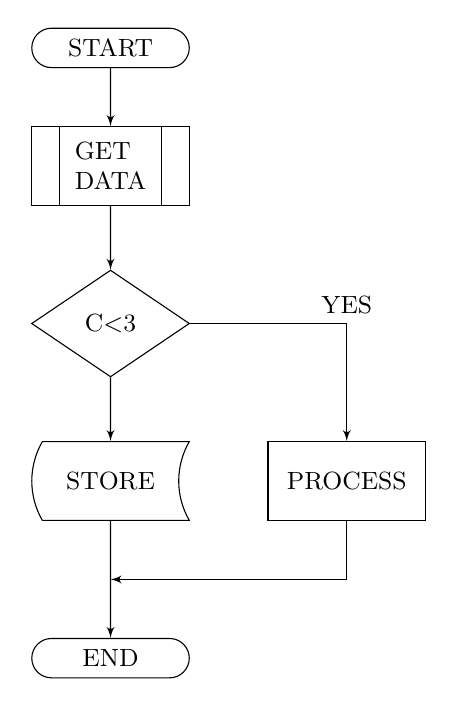
\begin{tikzpicture}[>=latex',font={ \small}]
\def\smbwd{2cm}
\node (terminal1) at (0,0) [draw, terminal,
minimum width=\smbwd,
minimum height=0.5cm] {START};
\node (predproc1) at (0,-1.5) [draw, predproc, align=left,
minimum width=\smbwd,
minimum height=1cm] {GET\\ DATA};
\node (decide1) at (0,-3.5) [draw, decision,
minimum width=\smbwd,
minimum height=1cm] {C$<$3};
\node (storage1) at (0,-5.5) [draw, storage,
minimum width=\smbwd,
minimum height=1cm] {STORE};
\node (process1) at (3,-5.5) [draw, process,
minimum width=\smbwd,
minimum height=1cm] {PROCESS};
\coordinate (point1) at (0,-6.75);
\node (terminal2) at (0,-7.75) [draw, terminal,
minimum width=\smbwd,
minimum height=0.5cm] {END};
\draw[->] (terminal1) -- (predproc1);
\draw[->] (predproc1) -- (decide1);
\draw[->] (decide1) -| node[above]{YES} (process1);
\draw[->] (decide1) -- (storage1);
\draw[->] (process1) |- (point1);
\draw[->] (storage1) -- (point1) -- (terminal2);
\end{tikzpicture}

\pgfornament[width=2cm,opacity=0.5,ydelta=9pt,symmetry=v,color=green!20!black]{25}

\begin{tikzpicture}
\tikzset{pgfornament/.style={
fill=green!60,fill opacity=.5,line width=1pt
}}
\pgfornament[color=red!20,scale=2,anchor=south]{24}
\end{tikzpicture}



\begin{tikzpicture}
\tikzset{pgfornamentstyle/.style={draw=red!40,fill=green!20}}
\node[draw=red!20,anchor=center,inner sep=0pt,fill=green!80!yellow] at (0,0){
\pgfornament[color=red!20,scale=2,anchor=south]{24}
};
\end{tikzpicture}

%\makeatletter%加入页脚装饰
%\AddToShipoutPicture{
%\begingroup
%\setlength{\@tempdima}{2mm}
%\setlength{\@tempdimb}{\paperwidth-\@tempdima-2cm}
%\setlength{\@tempdimc}{\paperheight-\@tempdima}
%\put(\LenToUnit{\@tempdima},\LenToUnit{\@tempdimc}){
%  \pgfornament[anchor=north west,width=2cm,color=Maroon]{41}}
%\put(\LenToUnit{\@tempdima},\LenToUnit{\@tempdima}){
%  \pgfornament[anchor=south west,width=2cm,symmetry=h,color=Maroon]{41}}
%\put(\LenToUnit{\@tempdimb},\LenToUnit{\@tempdimc}){
%  \pgfornament[anchor=north east,width=2cm,symmetry=v,color=Maroon]{41}}
%\put(\LenToUnit{\@tempdimb},\LenToUnit{\@tempdima}){
%  \pgfornament[anchor=south east,width=2cm,symmetry=c,color=Maroon]{41}}
%\endgroup
%}
%\makeatother
%\makeatletter
%\let\strippt\strip@pt
%\makeatother
%\newcommand{\zh}{
%\unitlength=1pt
%\begin{picture}(0,0)
%\put(0,0){\pgfornament[width=1cm]{41}};
%\put(\strippt\textwidth,0){
%   \pgfornament[width=1cm,symmetry=v]{41}};
%\put(0,-\strippt\textheight){
%   \pgfornament[width=1cm,symmetry=h]{41}};
%\put(\strippt\textwidth,-\strippt\textheight){
%   \pgfornament[width=1cm,symmetry=c]{41}};
%\end{picture}
%}限制角落装饰在text area里面,而不是paper area
\newcommand{\chh}{
\begin{tikzpicture}[remember picture,overlay]
  \node[anchor=north west] at (current page.north west){
                \pgfornament[width=2cm]{63}};
  \node[anchor=north east] at (current page.north east){
                \pgfornament[width=2cm,symmetry=v]{63}};
  \node[anchor=north west] at (current page.south west){
                \pgfornament[width=2cm,symmetry=h]{63}};
  \node[anchor=north west] at (current page.south west){
                \pgfornament[width=2cm,symmetry=c]{63}};
\end{tikzpicture}
}\newpage

%\AddToShipoutPictureFG{\pgfornament[scale=0.4,color=Maroon]{32}}



%\begin{tikzpicture}[remember picture,overlay]
%  \node[anchor=north west] at (current page.north west){
%                \pgfornament[width=2cm]{63}};
%  \node[anchor=north east] at (current page.north east){
%                \pgfornament[width=2cm,symmetry=v]{63}};
%  \node[anchor=south west] at (current page.south west){
%                \pgfornament[width=2cm,symmetry=h]{63}};
%  \node[anchor=south east] at (current page.south east){
%                \pgfornament[width=2cm,symmetry=c]{63}};
%\end{tikzpicture}

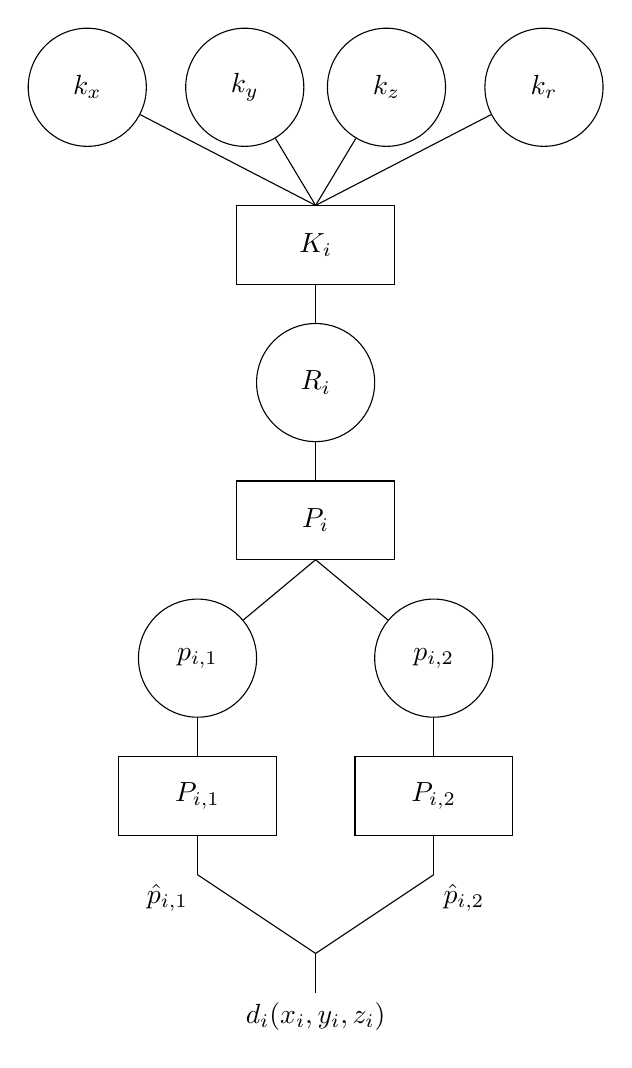
\begin{tikzpicture}
\node[rectangle](ki) at (0,0) [draw,
minimum width=2cm,
minimum height=1cm] {$K_i$};
\node[circle](ky) at (-0.9,2) [draw,
minimum width=1.5cm,
minimum height=1.5cm] {$k_y$};
\node[circle](kz) at (0.9,2) [draw,
minimum width=1.5cm,
minimum height=1.5cm] {$k_z$};
\node[circle](kx) at (-2.9,2) [draw,
minimum width=1.5cm,
minimum height=1.5cm] {$k_x$};
\node[circle](kr) at (2.9,2) [draw,
minimum width=1.5cm,
minimum height=1.5cm] {$k_r$};
\coordinate (pt) at (0,0.5);
\node[circle](ri) at (0,-1.75) [draw,
minimum width=1.5cm,
minimum height=1.5cm] {$R_i$};
\node[rectangle](pi) at (0,-3.5) [draw,
minimum width=2cm,
minimum height=1cm] {$P_i$};
\node[circle](pi1) at (-1.5,-5.25) [draw,
minimum width=1.5cm,
minimum height=1.5cm] {$p_{i,1}$};
\node[circle](pi2) at (1.5,-5.25) [draw,
minimum width=1.5cm,
minimum height=1.5cm] {$p_{i,2}$};
\node[rectangle](Pi2) at (1.5,-7) [draw,
minimum width=2cm,
minimum height=1cm] {$P_{i,2}$};
\node[rectangle](Pi1) at (-1.5,-7) [draw,
minimum width=2cm,
minimum height=1cm] {$P_{i,1}$};
\coordinate (pt1) at (-1.5,-8);
\coordinate (pt2) at (1.5,-8);
\node[anchor=north east] at (pt1) {$\hat p_{i,1}$};
\node[anchor=north west] at (pt2) {$\hat p_{i,2}$};
\coordinate (pt3) at (0,-9);\coordinate (pt4) at (0,-9.5);
\node[anchor=north] at (pt4) {$d_i(x_i,y_i,z_i)$};
\coordinate (pii) at (0,-4);
\draw[-] (kx)--(pt);
\draw[-] (ky)--(pt);
\draw[-] (kz)--(pt);
\draw[-] (kr)--(pt);
\draw[-] (ki)--(ri);
\draw[-] (ri)--(pi);
\draw[-] (pii)--(pi1);
\draw[-] (pii)--(pi2);
\draw[-] (pi1)--(Pi1);
\draw[-] (pi2)--(Pi2);
\draw[-] (Pi1)--(pt1);
\draw[-] (Pi2)--(pt2);
\draw[-] (pt1)--(pt3);\draw[-] (pt2)--(pt3);
\draw[-] (pt3)--(pt4);
\end{tikzpicture}
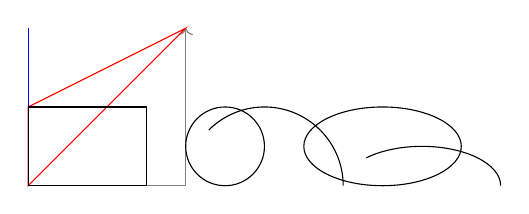
\begin{tikzpicture}
\coordinate (S) at (2,2);
\draw[gray,->] (0,0)-|(S);
\draw[blue] (0,0)--(0,0|-S);
\draw[red,->] (0,0)--(0,1)--(S)--cycle (0,1)--(1,1);
\draw(0,0)rectangle(1.5,1);
\draw(2.5,0.5)circle[radius=0.5];
\draw(4.5,0.5)ellipse[x radius=1,y radius=0.5];
\draw(4,0)arc(0:135:1);
\draw(6,0)arc(0:135:1 and 0.5);
\end{tikzpicture}


\tikz\draw[Latex-](0,0)--(1,0);
\tikz\draw[-Stealth](0,1)--(1,1);%\tikz[thick/very thick/ultra thick]\draw[-Stealth](0,1)--(1,1);
\tikz\draw[{Latex[]Stealth[]}-{Stealth[]Latex[]}](0,0)--(2,0);
\tikz[thin] \draw[-{Stealth[red]}](0,0)--(1,0);
\tikz[very thick] \draw[red,-Stealth](0,0)--(1,0);
\tikz[ultra thick] \draw[-{Stealth[length=6mm]}](0,0)--(1,0);
\tikz[semithick] \draw[-{Stealth[length=0pt 5]}](0,0)--(1,0);%箭头长度=0pt+当前线宽的5倍
\tikz\draw[-{Stealth[width=0pt 5]}](0,0)--(1,0);
\tikz\draw[-{Stealth[width'=2pt .5]}](0,0)--(1,0);%箭头宽度是长度的一半
\tikz\draw[-{Stealth[width'=2pt .5,open]}](0,0)--(1,0);%open空心箭头
\tikz\draw[-{Stealth[scale=2]}](0,0)--(1,0);%scale缩放比例
\tikz[ultra thick,foo/.tip={Stealth[red]}] \draw[-foo](0,0)--(1,0);%自定义箭头
\tikz[>=Stealth] \draw[<->](0,0)--(1,0);%>=等价于<->/.tip
\tikz\draw[red](0,0)-|(1,1);
\tikz\filldraw[fill=yellow,draw=blue](2,0.5)circle[radius=0.5];
\tikz\draw[blue](0,0)rectangle(1,1);
\tikz\draw[line width=12,rotate=30](0,0)--(2,0);
\tikz\draw[(-)](0,0)--(1,0);
\tikz\draw[*-*](0,0)--(1,0);
\tikz\draw[o-o](0,0)--(1,0);
\tikz\draw[-Hooks](0,0)--(1,0);
\tikz\draw[-{Stealth[reversed]}](0,0)--(1,0);
\tikz\draw[-{Stealth[harpoon]}];
\tikz\draw[-{Stealth[harpoon,swap]}];
\tikz\draw[-{Stealth[right]}];
\tikz[ultra thick]\draw[draw=red,fill=cyan,-{Stealth[length=10pt]}]
(0,0)--(1,1)--(2,0);

\tikz\draw[dashed](0,0)--(0,2);
\tikz\draw[dotted,-{Stealth[width=0pt 5]}](0,0)--(1,0);
\tikz\draw[loosely dash dot,-{Stealth[width=0pt 5]}](0,0)--(0,1)--(1,0)--cycle;
%dashed,dotted,dash dot和dash dot dot都有dendely和loosely类型
\tikz\draw[->>](0,0)--(1,0);\tikz\draw[>->|](0,0)--(1,0);
\tikz\draw[{latex}-{stealth}](0,0)--(2,0);\tikz\draw[-{to}|](0,0)--(1,0);
\tikz\draw(2,0)--(2,1)[rounded corners=.3cm]--(3,1)--(3.5,0)[sharp corners]--cycle;
\tikz{
\node[draw](A){$A$};
\node[draw](B)[right=of A]{$B$};
\draw[-{>>[sep=6pt]}](A)to[bend left =45](B);
\draw[-{>Stealth[sep=15pt]>}](A)to[bend right=45](B);
\draw[-{[sep=6pt]>>}](A)to(B);
}
\tikz\draw[-{Stealth[].Stealth[].Stealth[]}](0,0)--(2,0);
\tikz[Bar-{Stealth[sep=10pt]}]{
\draw(0,0)to[bend left](1,1);\draw(0,-0.5)--++(1,0);
}

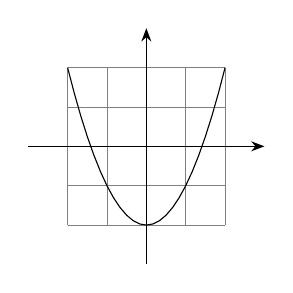
\begin{tikzpicture}[>=Stealth]
\draw[help lines,step=0.5](-1,-1)grid(1,1);
\draw[->](-1.5,0)--(1.5,0);
\draw[->](0,-1.5)--(0,1.5);
\draw[domain=-1:1]plot(\x,{\x*\x*2-1});
\end{tikzpicture}

\fbox{\parbox{0.5\textwidth}{%用scale/xshift/yshift/xslant/yslant/rotate设定图形的缩放,位移和旋转
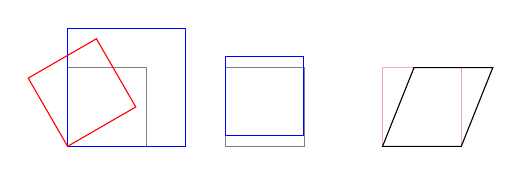
\begin{tikzpicture}
\draw[help lines](0,0) rectangle (1,1);
\draw[scale=1.5,blue] (0,0) rectangle (1,1);
\draw[rotate=30,red] (0,0) rectangle (1,1);
\draw[help lines] (2,0) rectangle (3,1);
\draw[yshift=4pt,blue] (2,0) rectangle (3,1);
\draw[pink](4,0) rectangle (5,1);
\draw[xslant=0.4](4,0) rectangle (5,1);
\end{tikzpicture}
}}%%%给环境整体加框的时候,用parbox封装

\tikzstyle{arrow}=[thick,->,>=stealth]%定义样式
\tikz\draw[arrow](0,0--(1,0)--(2,0);

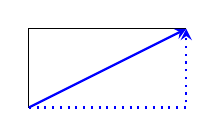
\begin{tikzpicture}[myarrow/.style={blue,thick,-stealth}]%定义样式
\draw (0,0)--(0,1)--(2,1);
\draw[myarrow](0,0)--(2,1);
\draw[myarrow,dotted](0,0)--(2,0)--(2,1);
\end{tikzpicture}
\subsection{}

\tikzset{box/.style={rectangle,draw=red!60,fill=blue!30}}
\begin{tikzpicture}
\node[box](tex)at(0,0){.tex};
\node[box](pdf)at(8,0){.pdf};
\node[box](dvi)at(4,2){.dvi};
\draw[-stealth](tex)--node[below]{pdflatex}(pdf);
\draw[-stealth](tex)--node[above,sloped]{latex}(dvi);
\draw[-stealth](dvi)--node[above right]{dvipdfmx}(pdf);
\node[rectangle](tex1) at (0,-4) [draw,
minimum width=0.25cm,
minimum height=0.5cm] {.tex};
\node[rectangle](pdf1) at (8,-4) [draw,
minimum width=0.25cm,
minimum height=0.5cm] {.pdf};
\node[rectangle](dvi1) at (4,-2) [draw,
minimum width=0.25cm,
minimum height=0.5cm] {.dvi};
\end{tikzpicture}
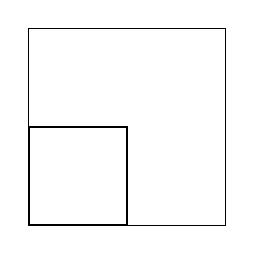
\begin{tikzpicture}
\draw(0,0) rectangle (2.5,2.5);
\begin{scope}[thick,scale=0.5]%scope环境使得参数只在局部生效
\draw(0,0)rectangle (2.5,2.5);
\end{scope}
\end{tikzpicture}
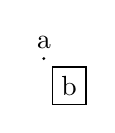
\begin{tikzpicture}
\coordinate (A) at (1,1);
\fill(A)circle(0.02);
\node[anchor=south] at (A){a};
\node[draw,below right=4pt]at(A){b};
\end{tikzpicture}
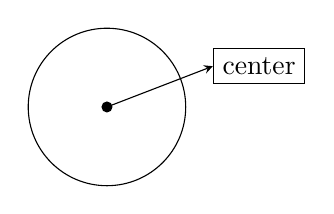
\begin{tikzpicture}
\draw (0,0)circle[radius=1];
\fill(0,0) circle[radius=2pt];
\node[rectangle](P) at(15:2)[draw]{center};
\draw[-stealth](0,0)--(P.west);
\end{tikzpicture}

\tikz\draw(2,1.5) node[above]{$A$}--node[above left]{$c$}(0,0)node[below]{$B$}
--node[below=2pt]{$a$}(2.5,0)node[below]{$C$}--node[above right]{$b$}cycle;
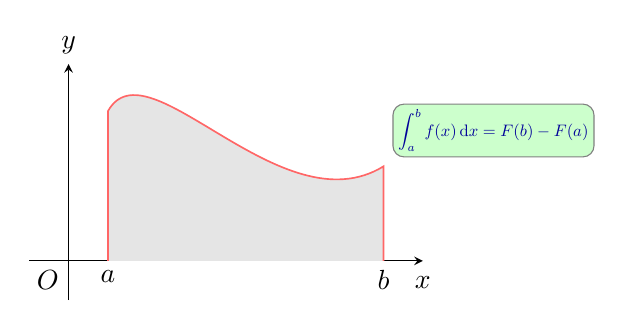
\begin{tikzpicture}
\draw[-stealth,line width=0.4pt](-0.5,0)--(4.5,0)node[below=2pt]{$x$};
\draw[-stealth,line width=0.4pt](0,-0.5)--(0,2.5)node[above]{$y$};
\coordinate(a) at(0.5,1.9);
\coordinate(b)at(4,1.2);
\draw[semithick,red](0.5,0.1)--(4,0.1);
\node[below](a0)at(a|-0,0){$a$};
\node[below](b0)at(b|-0,0){$b$};
\node[below left](O)at(0,0){$O$};
\filldraw[fill=gray!20,draw=red!60,semithick]
(a0)--(a)..controls(1,2.8)and(2.7,0.4)..(b)--(b0)--cycle;
\node[above right,outer sep=0.2cm,rounded corners,fill=green!20,draw=gray,text=blue!60!black,scale=0.6]
at(b){$\displaystyle\int_a^bf(x)\,\mathrm dx=F(b)-F(a)$};
\end{tikzpicture}

%抛物线,bend控制顶点。二次和三次Bezier曲线,分别用一个和两个控制点
\begin{tikzpicture}
\draw(0,0)parabola(1,2);
\draw(2,0)parabola bend(2.25,-0.25)(3,2);\fill(2.25,-0.25) circle(1pt)(4.75,2.25)circle(1pt);
\draw(4,0)parabola bend(4.75,2.25)(5,2);
\end{tikzpicture}
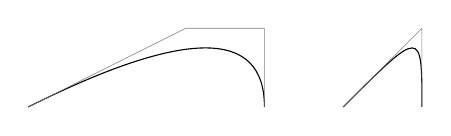
\begin{tikzpicture}
\draw(0,0)..controls(2,1)and(3,1)..(3,0);
\draw(4,0)..controls(5,1)..(5,0);
\draw[help lines](0,0)--(2,1)--(3,1)--(3,0)(4,0)--(5,1)--(5,0);
\end{tikzpicture}


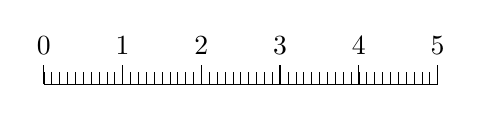
\begin{tikzpicture}
\draw(0,0)--(5,0);
\foreach \i in {0.0,0.1,...,5.0}
{\draw[very thin](\i,0)--(\i,0.15);}
\foreach \I in{0,1,2,3,4,5}
{\draw(\I,0)--(\I,0.25) node[above]{$\I$};}
\end{tikzpicture}
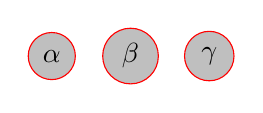
\begin{tikzpicture}
\foreach \n/\t in {0/\alpha,1/\beta,2/\gamma}{\node[circle,fill=lightgray,draw=red]at(\n,0){$\t$};}
\end{tikzpicture}

\tikzpicture
\draw(0,1)--($(0,1)-3*(-1,1)$);\draw(2,1)--++(1,-1)--++(1,1);\draw(3,1)--+(3,-1)--+(3,1);
\endtikzpicture
\tikz{\draw(0,0) to[out=60,in=-90](4,0);\draw(0,0)to(4,0);}%连接两点的曲线可以指定起始角度


\begin{tikzpicture}%%\shade是渐变命令
\shade[inner color=yellow,outer color=orange](1,1)circle[radius=1.3];%可以直接circle(1.3)
\shade[left color=gray,right color=red](3,0)rectangle(6,2);
\shade[top color=gray,bottom color=red](6,0)rectangle(9,2);
\end{tikzpicture}
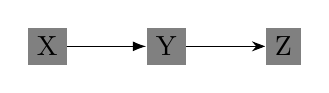
\begin{tikzpicture}%%载入positioning库,可以使用相对位置
\node[fill=gray](a){X};
\node[fill=gray,right=1 of a](b){Y};
\node[fill=gray,right=1 of b](c){Z};
\draw[-Latex](a)--(b);\draw[-Stealth](b)--(c);
\end{tikzpicture}%%%%%smooth选项用于绘制光滑曲线,tesion选项表示曲线的绷紧度
\tikz{\draw plot coordinates{(0,0)(1,2)(2,1)(4,3)};
\draw[color=red]plot[smooth]coordinates{(0,0)(1,2)(2,1)(4,3)}}

\tikz{\draw[color=red]plot[smooth,tension=0.9]coordinates{(0,0)(1,2)(2,1)(4,3)}}

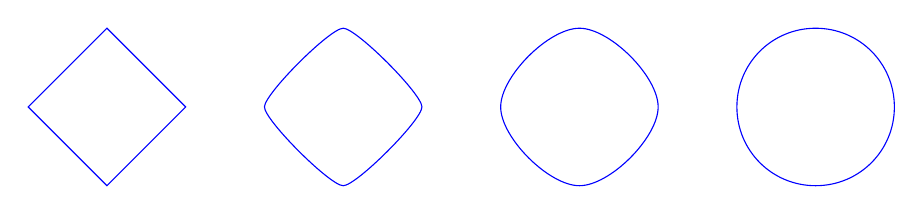
\begin{tikzpicture}[smooth cycle,blue]
\draw plot[tension=0]coordinates{(0,1)(1,0)(2,1)(1,2)};
\draw[xshift=3cm]plot[tension=0.3]coordinates{(0,1)(1,0)(2,1)(1,2)};
\draw[xshift=6cm]plot[tension=0.7]coordinates{(0,1)(1,0)(2,1)(1,2)};
\draw[xshift=9cm]plot[tension=1]coordinates{(0,1)(1,0)(2,1)(1,2)};
\end{tikzpicture}

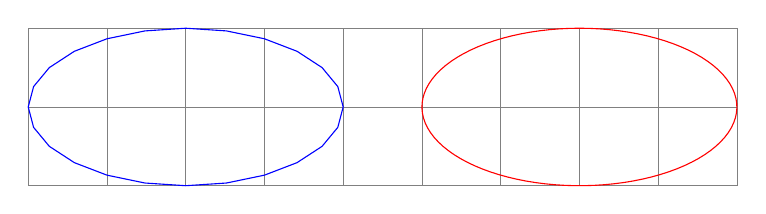
\begin{tikzpicture}[domain=0:2*pi]%%samples默认25,取点数越多,曲线越光滑
\draw[very thin,gray](-2,-1)grid(7,1);
\draw[blue]plot({2*sin(\x r)},{cos(\x r)});
\draw[red,samples=100]plot({5+2*sin(\x r)},{cos(\x r)});
\end{tikzpicture}

\newcommand\tikzmark[1]{
\tikz[overlay,remember picture]\node[coordinate](#1){};%
}%%%这里的%可以用于去掉多余的空格
这\tikzmark{a}个是一个重要的极限公式:
\[\tikzmark{b}\,\boxed{\lim_{x\to\infty}\left(1+\frac1x\right)^x=\mathrm e.}\]
\begin{tikzpicture}[overlay,remember picture]
\draw[-Stealth](a)..controls+(2em,-3em)..(b);
\draw[-Stealth](a)--(b);
\end{tikzpicture}

\begin{tikzpicture}[x={(-.1cm,-.15cm)},y={(1cm,0cm)},z={(0cm,1cm)}]
\draw[-Stealth](-5,0,0)--(5,0,0)node[below]{$x$};
\draw[-Stealth](0,-2,0)--(0,2,0)node[right]{$y$};
\draw[-Stealth](0,0,-1)--(0,0,3)node[above]{$z$};
\draw[red]plot[domain=0:2*pi]({sin(\x r)},{cos(\x r)},2);
\draw[red](0,0,0)--(0,1,2)(0,0,0)--(0,-1,2);
\end{tikzpicture}
%韦恩图venn - 两个圆相交
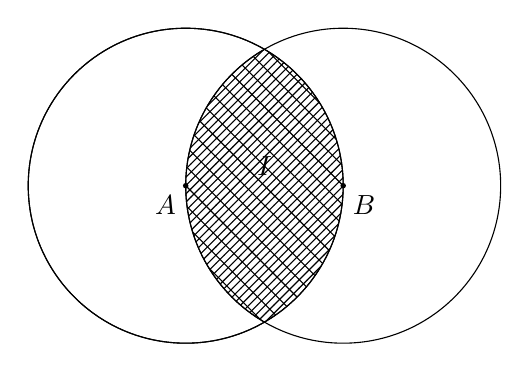
\begin{tikzpicture}
%\draw[-stealth](-2.5,0)--(4.5,0)node[right]{$x$};\draw[-stealth](0,-2.5)--(0,2.5)node[above]{$y$};
%%\draw[step=0.5cm,help lines](-2.5,-2.5)grid(4.5,2.5);
%\foreach \i in {0.0,0.5,...,5.5}
%{\draw[very thin](\i-2,0)--(\i-2,0.1);}
%\foreach \I in{-2,-1,0,1,2,3,4}
%{\draw[thick](\I,0)--(\I,0.2) node[below=4pt]{$\I$};}
    \draw (0,0)node[below left]{$A$} circle (2cm);\fill[black](0,0)circle(1pt);
    \draw (2,0)node[below right]{$B$} circle (2cm);\fill[black](2,0)circle(1pt);
    \clip[draw] (0,0) circle (2cm);
    \clip[draw] (2,0) circle (2cm);
    \foreach \x in {-1,-0.75,...,2.75}
    \draw[xshift=\x cm]  (-2,2)--(2,-2);
    \fill[pattern=north east lines](0,0)circle(2cm);
    \node[above] at (1,0) {$I$};
\end{tikzpicture}

%韦恩图venn - 3个圆相交
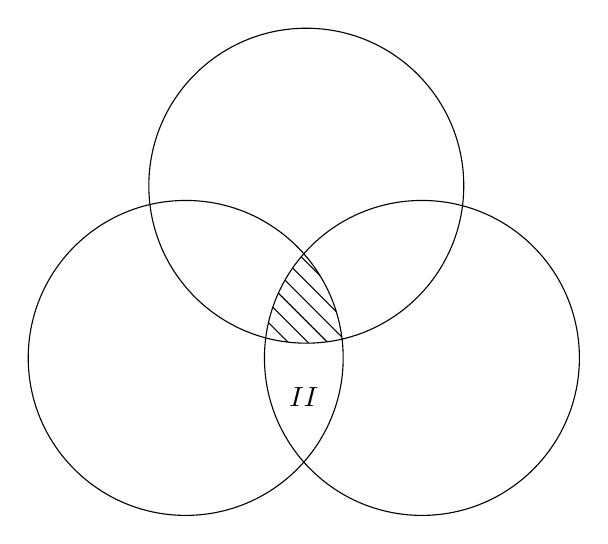
\begin{tikzpicture}
    \draw (0,0) circle (2cm);
    \draw (55:2.67cm) circle (2cm);
    \draw (0:3cm) circle (2cm);
    \begin{scope}
        \clip (0,0) circle (2cm);
        \clip (55:2.67cm) circle (2cm);
        \clip (0:3cm) circle (2cm);
        \foreach \x in {-1,-0.75,...,2.75}
        \draw[xshift=\x cm]  (-2,2)--(2,-2);
    \end{scope}
    \node at (1.5,-0.5) {$II$};
\end{tikzpicture}
%韦恩图venn - 3个圆相交(斜线填充)
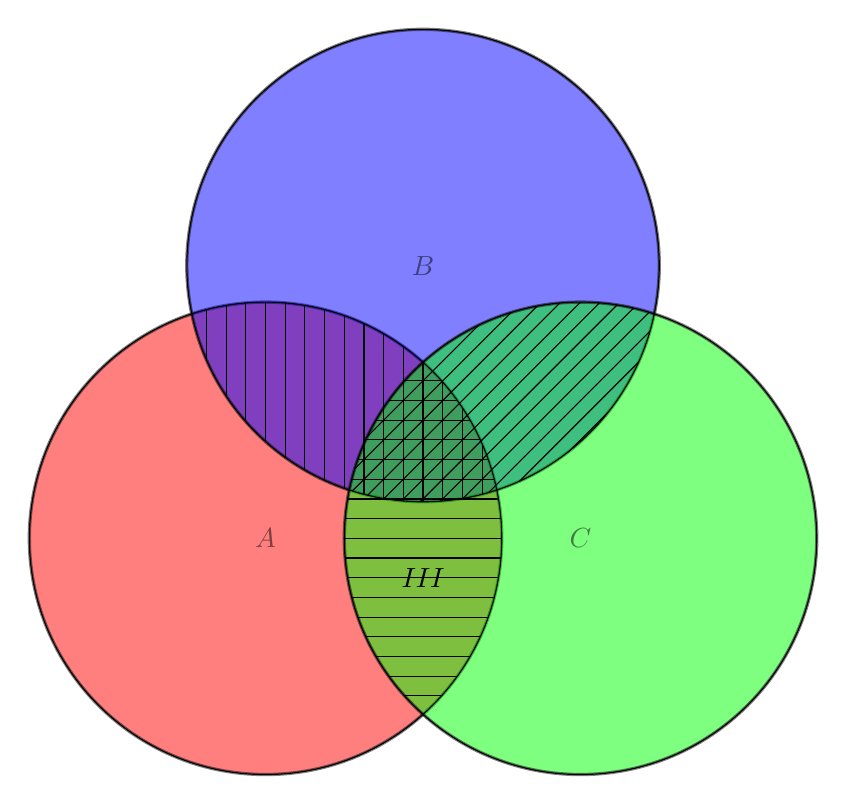
\begin{tikzpicture}  %用[scale=0.8]出问题!
    \tikzset{venn circle/.style={draw,circle,minimum width=6cm,fill=#1,opacity=0.5,very thick}}
    \node [venn circle = red] (A) at (0,0) {$A$};
    \node [venn circle = blue] (B) at (60:4cm) {$B$};
    \node [venn circle = green] (C) at (0:4cm) {$C$};
    \draw (0,0) circle (3cm);
    \draw (60:4cm) circle (3cm);
    \draw (0:4cm) circle (3cm);
    \begin{scope}
    \clip (0,0) circle (3cm);
    \clip (60:4cm) circle (3cm);
    \foreach \x in {-5,-4.75,...,5,5}
    \draw[overlay, xshift=\x cm]  (2,4)--(2,0);
    \end{scope}
    \begin{scope}
    \clip (60:4cm) circle (3cm);\clip (0:4cm) circle (3cm);
    \foreach \y in {-5,-4.75,...,5}
    \draw[overlay, xshift=\y cm]  (1,0)--(5,4);
    \end{scope}
    \begin{scope}
    \clip (0,0) circle (3cm);
    \clip (0:4cm) circle (3cm);
    \foreach \z in {-5,-4.75,...,5}
    \draw[overlay, yshift=\z cm]  (0,3)--(4,3);
    \end{scope}
    \node at (2,-0.5) {$III$};
\end{tikzpicture}

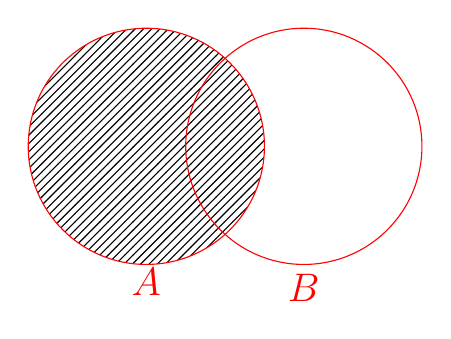
\begin{tikzpicture}[red,every node/.style={font=\Large}]
\draw[pattern=north east lines] (0,0) circle(1.5);
\draw (2,0) circle(1.5);
\node[fill=white,inner sep=1pt,rounded corners,below=3] at (90:1.5) {$A$};
\node[xshift=2cm,below=3] at (90:1.5) {$B$};
\end{tikzpicture}

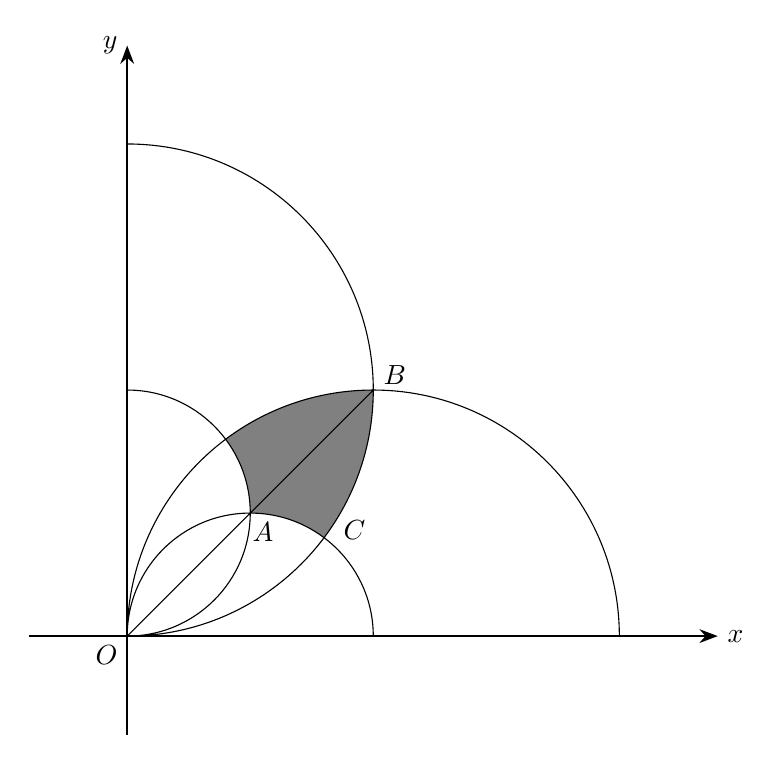
\begin{tikzpicture}[scale=25]
\begin{scope}
\clip (0,0) arc (-90:0:1/8) arc (90:180:1/8);
\fill[gray,even odd rule] (0,0) arc (-90:0:1/8) arc (90:180:1/8)
arc (-90:270:1/16) arc (-180:180:1/16) arc (-90:0:1/16) arc (90:180:1/16);
\end{scope}
\node[below left](0,0){$O$};
\draw [-Stealth,thick](-0.05,0)--(0.3,0);\draw [-Stealth,thick](0,-0.05)--(0,0.3);
\node[right]at(0.3,0){$x$};\node[left]at(0,0.3){$y$};
\draw (0,0) arc (-90:90:1/8) (0,0) arc (-90:90:1/16)
(0,0) arc (180:0:1/8) (0,0) arc (180:0:1/16) (0,0)--(1/8,1/8);
\node [below]at(0.069,0.0627){$A$};
\node [above]at(0.136,0.123){$B$};
\node [right]at(0.105,0.0541){$C$};
\end{tikzpicture}
\begin{tikzpicture}[scale=25]
\begin{scope}
\clip (0,0) arc (-90:0:1/8) arc (90:180:1/8);
\fill[pattern=horizontal lines]
(0,0) arc (-90:0:1/8) --(1/16,1/16) arc (90:0:1/16);
\fill[pattern=vertical lines]
(0,0) arc (180:90:1/8) --(1/16,1/16) arc (0:90:1/16);
\end{scope}\node[below left](0,0){$O$};
\draw [-Stealth,thick](-0.05,0)--(0.3,0);\draw [-Stealth,thick](0,-0.05)--(0,0.3);
\node[right]at(0.3,0){$x$};\node[left]at(0,0.3){$y$};
\draw (0,0) arc (-90:90:1/8) (0,0) arc (-90:90:1/16)
(0,0) arc (180:0:1/8) (0,0) arc (180:0:1/16) (0,0)--(1/8,1/8);
\node [below]at(0.069,0.0627){$A$};
\node [above]at(0.136,0.123){$B$};
\node [right]at(0.105,0.0541){$C$};
\end{tikzpicture}

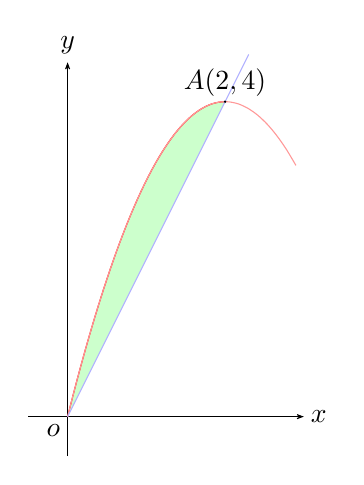
\begin{tikzpicture}[smooth]
\draw[arrows={-Stealth[length=5pt, inset=3.5pt]}] (-0.5,0) -- (3.0,0)node (xaxis) [right=-1pt] {$x$};
\draw[arrows={-Stealth[length=5pt, inset=3.5pt]}] (0,-0.5) -- (0,4.5)node (yaxis) [above=-0.6pt] {$y$};
\draw  (-0.18,-0.18) node {$o$};
\draw[color=red,domain=0:2.0,fill=green!20] plot (\x,4*\x-\x*\x);
\draw[color=red!40,domain=0:2.90] plot (\x,4*\x-\x*\x)  ;
\draw[color=blue!30,domain=0:2.3] plot (\x,2*\x)  ;
\draw[fill=black] (2,4) circle [radius=0.2pt] node[above=-1.8pt] {$A(2,4)$};
\end{tikzpicture}
 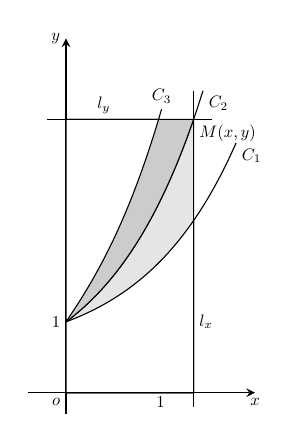
\begin{tikzpicture}[yscale=0.9,xscale=1.2]
    \draw[-stealth] (-0.4,0)--(2,0) node[below,scale=0.6]{$x$};
    \draw[-stealth] (0,-0.3)--(0,5) node[left,scale=0.6]{$y$};
    \draw (0,0) node [below left,scale=0.6] {$o$};
    \foreach \i in {1}{\draw (\i,0)--node [below,scale=0.6] {$1$}(\i,0.05);}
    \draw (0,1) node [left,scale=0.6] {$1$};
    \draw (1.35,1) node [right,scale=0.6] {$l_x$};
    \draw (0.4,3.85742) node [above,scale=0.6] {$l_y$};
    \draw (1.35,-0.2) -- (1.35,4.25519);
    \draw (-0.2,3.85742) -- (1.55,3.85742);
    \draw (1.35,3.85742) node [below right,scale=0.6] {$M(x,y)$};
    %\clip (-1,-1) rectangle (5,5);%只在这个区域内画图
    \draw[domain=1:4,smooth,variable=\t] plot ({ln(\t)+1/(2*\t)-0.5},\t)node[above,scale=0.6] {$C_3$};
    \draw[domain=0:1.8,smooth] plot (\x,{0.5*1+0.5*exp(\x)}) node[below right,scale=0.6] {$C_1$};
    \draw[domain=0:1.45,smooth] plot (\x,{exp(\x)}) node[below right,scale=0.6] {$C_2$};
    \filldraw [fill=gray!20] (0,0) -- plot [domain=0:1.35,smooth] (\x,{exp(\x)}) -- (1.35,0) -- (0,0);
    \filldraw [fill=white] (0,0) -- plot [domain=0:1.35,smooth] (\x,{0.5*1+0.5*exp(\x)}) -- (1.35,0) -- (0,0);
    \filldraw [fill=gray!40] (0,1) -- plot [domain=0:1.35,smooth] (\x,{exp(\x)}) -- (0,3.85742) -- (0,1);
    \filldraw [fill=white] (0,1) -- plot [domain=1:3.85742,smooth,variable=\t] ({ln(\t)+1/(2*\t)-0.5},\t) -- (0,3.85742) -- (0,1);
    \end{tikzpicture}
       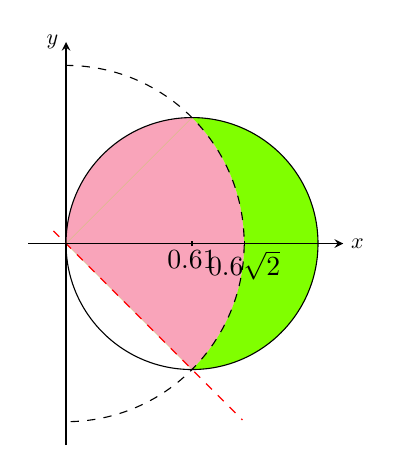
\begin{tikzpicture}[scale=1.6]
    \draw[-stealth] (-0.3,0) -- (2.2,0)node (xaxis) [right,scale=0.8] {$x$};
    \draw[-stealth] (0,-1.6) -- (0,1.6)node (yaxis) [left,scale=0.8] {$y$};
    \fill[pink!] (0,0) -- (1,-1) arc [start angle=315, end angle=405, radius=1.414] -- (0,0);
    \fill[pink!] (1,0) -- (1,1) arc [start angle=90, end angle=180, radius=1] -- (0,0);
    \fill[grassgreen] (0,0) -- (1,-1) arc [start angle=315, end angle=360, radius=1.414] -- (1.414,0)--(2,0) arc [start angle=360, end angle=270, radius=1] -- (1,-1);
    \fill[grassgreen] (0,0) -- (1,1) arc [start angle=45, end angle=0, radius=1.414] -- (1.414,0)--(2,0) arc [start angle=0, end angle=90, radius=1] -- (1,1);
    \draw (1,-0.02)--(1,0.02) node[below] {$\scaleobj{0.6}{1}$};
    \draw (1.414,-0.02)--(1.414,0.02) node[below] {$\scaleobj{0.6}{\sqrt{2}}$};
    \draw[style=dashed,color=red,domain=-0.1:1.4] plot(\x,-\x);
    \draw[color=black,domain=-0.1:2.2] plot(\x,0);
    \draw[style=dashed] (0,0)--(0,-1.414) arc [start angle=270, end angle=450, radius=1.414];
    \draw (1,0) circle [radius=1];
    %\fill[pattern=north west lines](0,0)--(-2,0)--(-2,2)--(0,2)arc(90:270:0.8);
    %\fill[pattern=north west lines]arc(-45:0:1);
    \end{tikzpicture}

    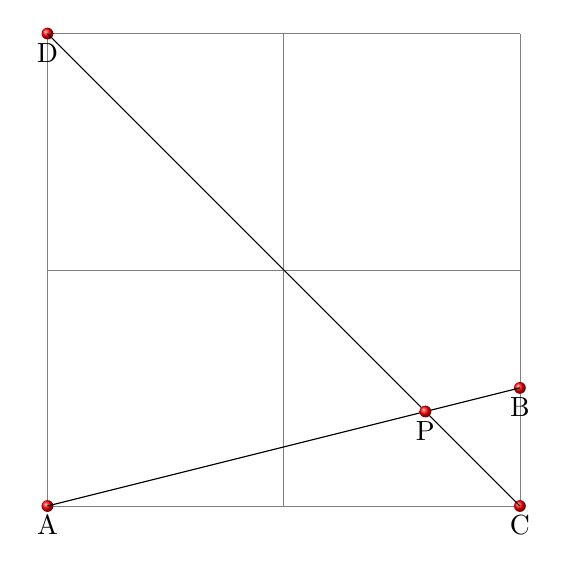
\begin{tikzpicture}[scale=3]
\draw[help lines] (0,0) grid (2,2);
\coordinate (A) at (0,0);
\coordinate (B) at (2,0.5);
\coordinate (C) at (2,0);
\coordinate (D) at (0,2);
\shade[ball color=red](A) circle (0.025) node[below] {A};
\shade[ball color=red](B) circle (0.025) node[below] {B};
\shade[ball color=red](C) circle (0.025) node[below] {C};
\shade[ball color=red](D) circle (0.025) node[below] {D};
\draw[name path=AB] (A) -- (B); \draw[name path=CD] (C) -- (D);
\path[name intersections={of=AB and CD}] (intersection-1) coordinate (P);
\shade[ball color=red](P) circle (0.025) node[below] {P};
\end{tikzpicture}
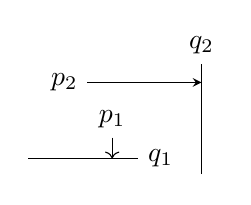
\begin{tikzpicture}
\node (p1) at (30:1) {$p_1$} ;
\node (p2) at (75:1) {$p_2$} ;
\draw (-0.2,0) -- (1.2,0) node[right] (xline) {$q_1$};
\draw (2,-0.2) -- (2,1.2) node[above] (yline) {$q_2$};
\draw[->] (p1) -- (p1 |- xline);
\draw[-stealth](p2)--(p2-|yline);
\end{tikzpicture}

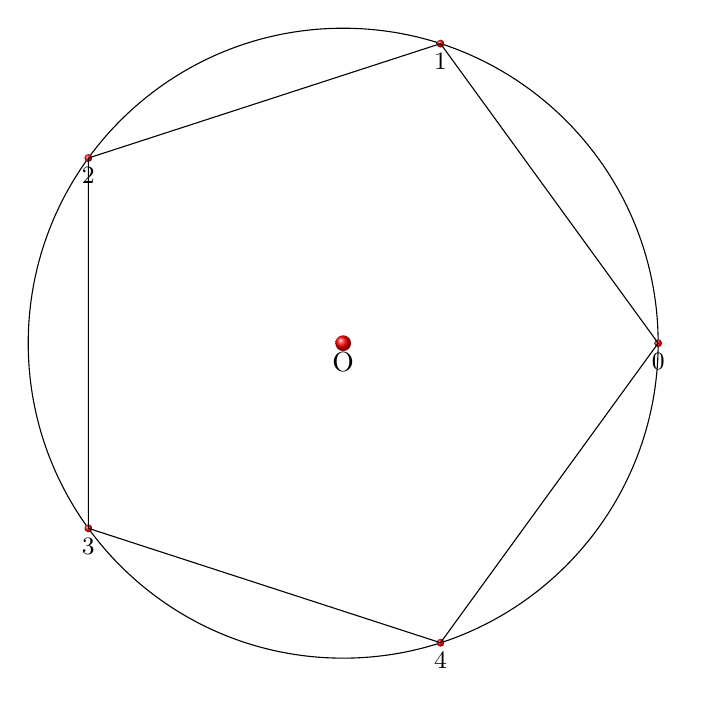
\begin{tikzpicture}
\draw (0,0) circle (4) ;
\coordinate (O) at (0,0);
\shade[ball color=red](O) circle (0.1) node[below] {O};
\def\n{5}
\pgfmathsetmacro\i{\n-1}
\foreach \x in {0,...,\i}
{
\def\pointname{\x}
\coordinate (\pointname) at ($(0,0) +(\x*360/\n:4cm)$)  ;
\shade[ball color=red](\pointname) circle (0.05) node[below] {\small \x};
}

\draw (0)
\foreach \x in {0,...,\i}
{ -- (\x) } -- cycle;

\end{tikzpicture}
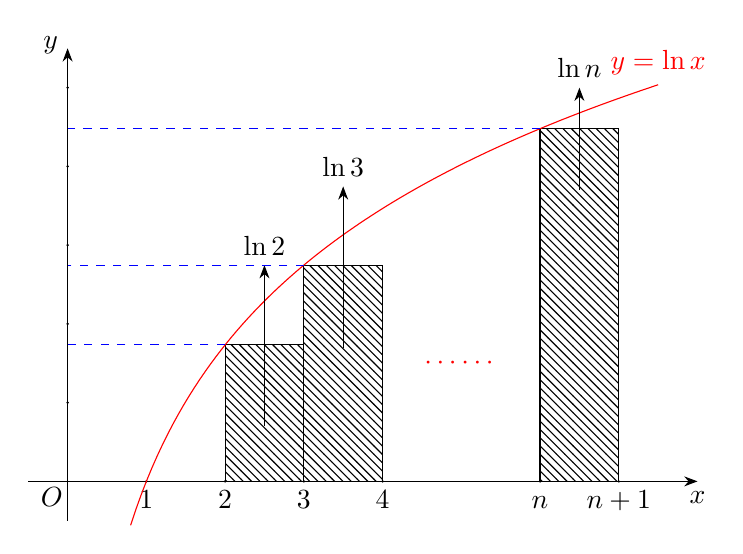
\begin{tikzpicture}
\draw[-Stealth](-0.5,0)--(8,0)node[below]{$x$};
\draw[-Stealth](0,-0.5)--(0,5.5)node[above=1pt,left]{$y$};
\node(O)at(-0.2,-0.2){$O$};
\foreach \i in{1,2,...,5}
{\draw[fill=blue](0,\i)circle(.2pt);}
\foreach \j in{1,2,3,4}
{\draw[fill=blue](\j,0)circle(.2pt)node[below]{$\j$};}
\draw[fill=blue](6,0)circle(.2pt)node[below=2pt]{$n$};
\draw[fill=blue](7,0)circle(.2pt)node[below]{$n+1$};
\node[red]at (5,1.5){$\cdots\cdots$};
\filldraw[pattern=north west lines](2,0)--(3,0)--(3,1.732868)--(2,1.732868)--cycle;
\filldraw[pattern=north west lines](3,0)--(4,0)--(4,2.7465)--(3,2.7465)--cycle;
\filldraw[pattern=north west lines](6,0)--(7,0)--(7,4.4794)--(6,4.4794)--cycle;
\draw[red,samples=100,domain=0.8:7.5]plot(\x,{2.5*ln(\x)})node[above]{$y=\ln x$};
\draw[-Stealth](2.5,0.7)--(2.5,2.7465)node[above]{$\ln2$};
\draw[-Stealth](3.5,1.7)--(3.5,3.7465)node[above]{$\ln3$};
\draw[-Stealth](6.5,3.7)--(6.5,5)node[above]{$\ln n$};
\draw[dashed,blue](2,1.732868)--(0,1.732868);
\draw[dashed,blue](3,2.7465)--(0,2.7465);
\draw[dashed,blue](6,4.4794)--(0,4.4794);
\end{tikzpicture}

\tikz {
\foreach \angle in {0,10,...,360}
\fill (canvas polar cs:angle=\angle,x radius=1cm,y radius=1.5cm)
circle (2pt);
}
\tikz{\node (start) [draw,ellipse] {start};
\foreach \angle in {-90, -80, ..., 90}
\draw (node cs:name=start,angle=\angle)..controls +(\angle:1cm) and +(-1,0)..(2.5,0);}
\begin{tikzpicture}[scale=2]%%samples默认25,取点数越多,曲线越光滑
\draw[-stealth](-1.2,0)--(1.2,0)node[right]{$p$};
\draw[-stealth](0,-0.3)--(0,1.2)node[above]{$E$};
\node[blue]at(-0.1,-0.1){$O$};
\draw[domain=-1.3:1.3,red,samples=40]plot({(\x)^3-\x},{3*(\x)^4/4-(\x)^2/2});
\end{tikzpicture}
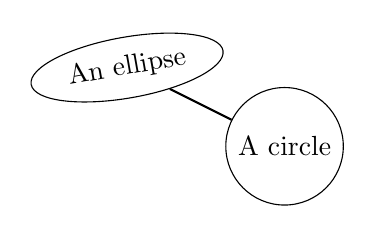
\begin{tikzpicture}
\path (0,0) node(a) [ellipse,rotate=10,draw]{An ellipse}
(2,-1) node(b) [circle,draw] {A circle};
\draw[thick] (a) -- (node cs:name=b);
\end{tikzpicture}

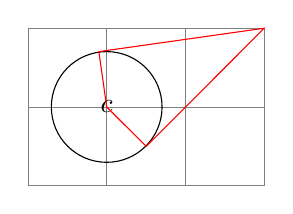
\begin{tikzpicture}%%%tangent坐标系
\draw[help lines] (0,0) grid (3,2);
\coordinate (a) at (3,2);
\node [circle,draw] (c) at (1,1) [minimum size=40pt] {$c$}; \draw[red] (a) -- (tangent cs:node=c,point={(a)},solution=1)
	--(c.center) -- (tangent cs:node=c,point={(a)},solution=2)
	--cycle;

\end{tikzpicture}
\begin{tikzpicture}
\draw[-stealth](0,0)--(6,0)node[below]{$x$};\node at(-0.2,-0.2){$O$};
\draw[-stealth](0,0)--(0,1.8)node[above]{$y$};
%\draw[red,samples=40,domain=0.001:2.8]plot(\x,{(\x)*ln(\x)})node[above]{$y=x\ln x$};
%\draw[blue,samples=40,domain=-1.8:0]plot(\x,{\x*abs(\x)})node[below=2.6cm,left]{$y=x|x|$};
\draw[blue,samples=60,domain=0:pi/2.25]plot({tan(\x r)},\x)node[above]{$y=\arctan x$};
\end{tikzpicture}
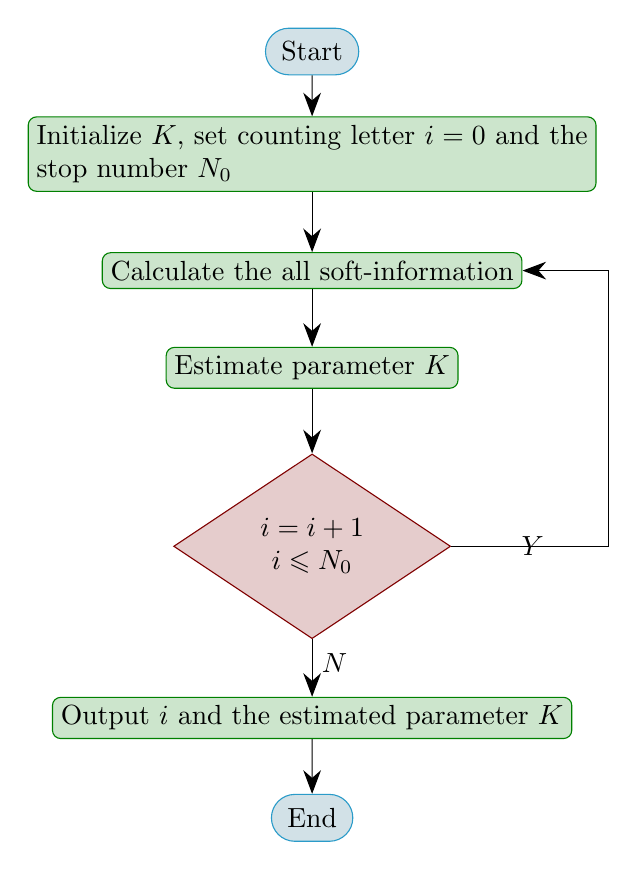
\begin{tikzpicture}
	\tikzset{
		start/.style ={
			rounded rectangle,
			inner sep=5pt,
			draw=cyan!80!black,
			fill=cyan!50!black!20},
		method/.style ={
			rectangle,
			rounded corners=3pt,
			inner sep=3pt,
			draw=green!50!black,
			fill=green!50!black!20},
		branch/.style ={
			diamond,
			aspect=1.5,
			draw=red!50!black,
			fill=red!50!black!20},
		>=stealth
	}
	\node(start) [start] {Start};
	\node(initial) at ([yshift=-1cm] start.south)[method]{\parbox{7cm}{Initialize $K$, set counting letter $i=0$ and the stop number $N_0$}};
	\node(soft) at ([yshift=-1cm] initial.south)[method]{Calculate the all soft-information};
	\node(estimated) at ([yshift=-1cm] soft.south)[method]{Estimate parameter $K$};
	\node(check) at ([yshift=-2cm] estimated.south)[branch]{$\begin{array}{c}
		i=i+1\\ i\leqslant N_0
		\end{array}$};
	\node(output) at ([yshift=-1cm] check.south)[method]{Output $i$ and the estimated parameter $K$};
	\node(end) at ([yshift=-1cm] output.south)[start]{End};
	\path[->,>={Stealth[length=3mm]}](start)edge(initial)
	(initial)edge(soft)
	(soft)edge(estimated)
	(estimated)edge(check)
	(check)edge(output)
	(output)edge(end);
	\coordinate (A) at ([xshift=2cm]check.east);
	\coordinate (B) at (A|-soft.east);
	\draw[->,>={Stealth[length=3mm]}](check.east)--(A)node[above,left=0.7cm]{$Y$}--(B)--(soft.east);
	\node at ([yshift=-3mm]check.south)[right]{$N$};
	\end{tikzpicture}
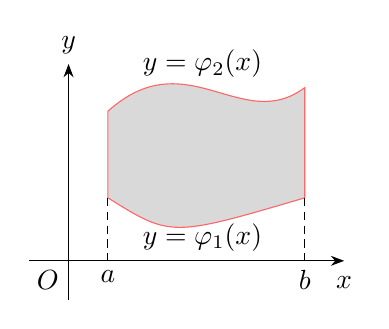
\begin{tikzpicture}
\draw[-Stealth,line width=0.4pt](-0.5,0)--(3.5,0)node[below=2pt]{$x$};
\draw[-Stealth,line width=0.4pt](0,-0.5)--(0,2.5)node[above]{$y$};
\coordinate(a) at(0.5,1.9);
\coordinate(b)at(3,2.2);
\coordinate(c)at(0.5,0.8);\coordinate(d)at(3,0.8);
\node[below](a0)at(a|-0,0){$a$};
\node[below](b0)at(b|-0,0){$b$};
\node[below left](O)at(0,0){$O$};
\filldraw[fill=gray!30,draw=red!60]
(c)--(a)..controls(1.5,2.8)and(2.2,1.6)..(b)--(d)..controls(1.3,0.3)..(c);
\node at(1.7,2.5){$y=\varphi_2(x)$};
\node at(1.7,0.3){$y=\varphi_1(x)$};
\draw[densely dashed](c)--(0.5,0);
\draw[densely dashed](d)--(3,0);
\end{tikzpicture}
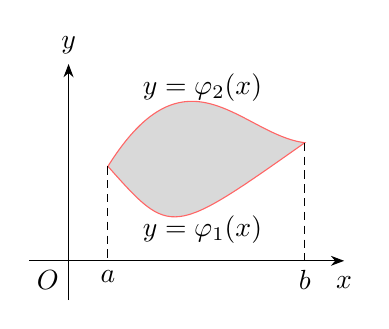
\begin{tikzpicture}
\draw[-Stealth,line width=0.4pt](-0.5,0)--(3.5,0)node[below=2pt]{$x$};
\draw[-Stealth,line width=0.4pt](0,-0.5)--(0,2.5)node[above]{$y$};
\coordinate(a) at(0.5,1.2);
\coordinate(b) at(3,1.5);
\node[below](a0)at(a|-0,0){$a$};
\node[below](b0)at(b|-0,0){$b$};
\node[below left](O)at(0,0){$O$};
\filldraw[fill=gray!30,draw=red!60]
(a)..controls(1.5,2.8)and(2.2,1.6)..(b)..controls(1.3,0.3)..(a);
\node at(1.7,2.2){$y=\varphi_2(x)$};
\node at(1.7,0.4){$y=\varphi_1(x)$};
\draw[densely dashed](a)--(0.5,0);
\draw[densely dashed](b)--(3,0);
\end{tikzpicture}
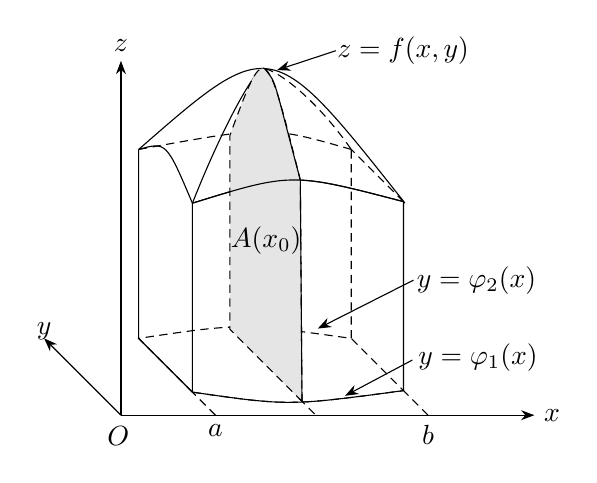
\begin{tikzpicture}
\begin{scope}[x={(1cm,0cm)},y={(-0.13cm,0.13cm)},z={(0cm,1cm)},scale=1.5]
\coordinate(O)at(0,0);
\node at(-0.1,-0.6,-0.1){{$O$}};
\draw[-Stealth,line width=0.4pt](0,0,0)--(0,5,0)node[above=-4pt]{{$y$}};
\draw[-Stealth,line width=0.4pt](0,0,0)--(0,0,3)node[above]{{$z$}};
\draw[-Stealth,line width=0.4pt](0,0,0)--(3.5,0,0)node[right]{{$x$}};
\coordinate(a) at(0.8,5,0);
\coordinate(b) at(2.6,5,0);
\coordinate(c) at(0.8,1.5,0);
\coordinate(d) at(2.6,1.6,0);
\node[below]at(0.8,0,0){{$a$}};
\node[below]at(2.6,0,0){{$b$}};
\draw[densely dashed]
(c)--(a)..controls(1.8,6,0)..(b)--(d)..controls(1.5,0.6,0)..(c);
\draw(a)--(c)..controls(1.5,0.6,0)..(d);
\draw(a)--(0.8,5,1.6);\draw(c)--(0.8,1.5,1.6);
\draw[densely dashed](b)--(2.6,5,1.6);\draw(d)--(2.6,1.6,1.6);
\draw(0.8,5,1.6)..controls(0.8,3.2,1.9)..(0.8,1.5,1.6)..controls(1.9,3.5,1.6)..(2.6,1.6,1.6);
\draw[densely dashed](2.6,5,1.6)..controls(1.9,5,1.8)..(0.8,5,1.6);
\draw(0.8,5,1.6)..controls(1.7,3.3,2.8)..(2.6,1.5,1.6);
\draw[densely dashed](2.6,1.6,1.6)--(2.6,5,1.6);
\draw(0.8,1.5,1.6)..controls(1.2,2.4,2.2)and(1.6,3.2,2.6)..(1.65,3.3,2.5);
\draw[densely dashed](1.65,3.3,2.5)..controls(1.7,3.3,2.51)and(2.15,4.2,2.2)..(2.6,5,1.6);
\filldraw[densely dashed,fill=gray!20](1.65,0.9,0)--(1.65,5.6,0)--(1.65,5.6,1.64)
..controls(1.65,3.3,2.75)..(1.75,1.78,1.76)--cycle;
\draw(0.8,1.5,1.6)..controls(1.9,3.5,1.6)..(2.6,1.6,1.6);
\draw[densely dashed](0.8,0,0)--(c)(2.6,0,0)--(d);
\draw(1.65,0.9,0)--(1.75,1.78,1.76)..controls(1.66,2.95,2.52)and(1.67,2.7,2.45)..(1.65,3.3,2.5);
\draw[densely dashed](1.65,1.1,0)--(1.65,0,0);
\end{scope}
\draw[-Stealth](5,6.9,5.9)node[right=-3pt]{{$z=f(x,y)$}}--(3.6,6,4.2);
\draw[-Stealth](4.1,2.1,1)--(2.5,1.1,0);
\node at(4.9,2.1,1){$y=\varphi_2(x)$};
\draw[-Stealth](3.7,0.7,0)--(3,0.4,0.4);
\node at(4.65,0.85,0.3){{$y=\varphi_1(x)$}};
\node at(2.23,2.6,1){$A(x_0)$};
\end{tikzpicture}

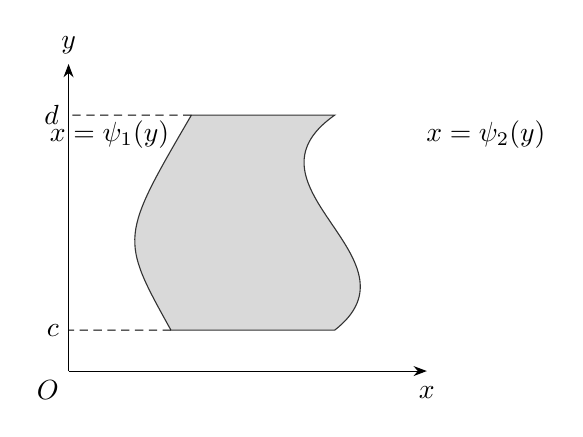
\begin{tikzpicture}
\begin{scope}[scale=1.3]
\draw[-Stealth,line width=0.4pt](0,0)--(3.5,0)node[below=2pt]{$x$};
\draw[-Stealth,line width=0.4pt](0,0)--(0,3)node[above]{$y$};
\coordinate(c) at(1,0.4);
\coordinate(d)at(1.2,2.5);
\coordinate(a)at(2.6,0.4);\coordinate(b)at(2.6,2.5);
\node[left](c0)at(c-|0,0){$c$};
\node[left](d0)at(d-|0,0){$d$};
\node[below left](O)at(0,0){$O$};
\filldraw[fill=gray!30,draw=black!80]
(c)--(a)..controls(3.5,1.1)and(1.6,1.8)..(b)--(d)..controls(0.5,1.3)..(c);
\draw[densely dashed](c)--(0,0.4);
\draw[densely dashed](d)--(0,2.5);
\end{scope}
\node at (0.52,3){$x=\psi_1(y)$};
\node at (5.3,3){$x=\psi_2(y)$};
\end{tikzpicture}
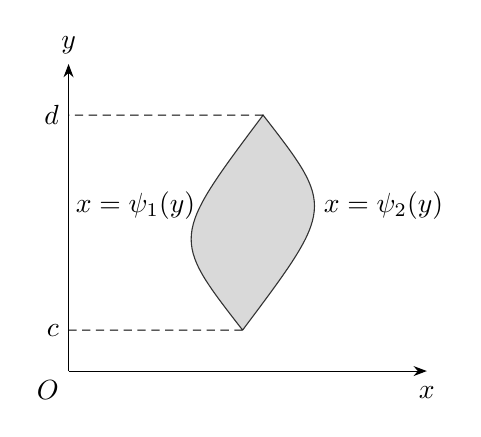
\begin{tikzpicture}
\begin{scope}[scale=1.3]
\draw[-Stealth,line width=0.4pt](0,0)--(3.5,0)node[below=2pt]{$x$};
\draw[-Stealth,line width=0.4pt](0,0)--(0,3)node[above]{$y$};
\coordinate(c) at(1.7,0.4);
\coordinate(d)at(1.9,2.5);
\node[left](c0)at(c-|0,0){$c$};
\node[left](d0)at(d-|0,0){$d$};
\node[below left](O)at(0,0){$O$};
\filldraw[fill=gray!30,draw=black!80]
(c)..controls(2.6,1.6)..(d)..controls(1,1.3)..(c);
\draw[densely dashed](c)--(0,0.4);
\draw[densely dashed](d)--(0,2.5);
\end{scope}
\node at (0.85,2.1){$x=\psi_1(y)$};
\node at (4,2.1){$x=\psi_2(y)$};
\end{tikzpicture}
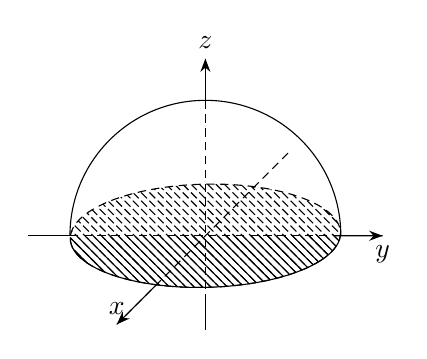
\begin{tikzpicture}
\begin{scope}[y={(1cm,0cm)},x={(-0.5cm,-0.5cm)},z={(0cm,1cm)},scale=1.5]
\draw[-Stealth,densely dashed,line width=0.4pt](0,-1.5,0)--(0,1.5,0)node[below]{{$y$}};
\draw[-Stealth,densely dashed,line width=0.4pt](0,0,-0.8)--(0,0,1.5)node[above]{{$z$}};
\draw[-Stealth,densely dashed,line width=0.4pt](-1.4,0,0)--(1.5,0,0)node[above]{{$x$}};
\filldraw[samples=100,densely dashed,rotate=-12,pattern=north west lines]plot[domain=0:2*pi]({sin(\x r)},{cos(\x r)},0);
\filldraw[samples=100,rotate=-12,pattern=north west lines]plot[domain=-pi/6:5*pi/6]({sin(\x r)},{cos(\x r)},0);
\draw(0,0,1.1)--(0,0,1.5)(0,0,-0.5)--(0,0,-0.8);
\draw(0.8,0,0)--(1.5,0,0)(0,1.1,0)--(0,1.5,0);
\draw(0,-1.5,0)--(0,-1.1,0);
\end{scope}
\draw(1.72,0)arc(0:180:1.72 and 1.72);
\end{tikzpicture}
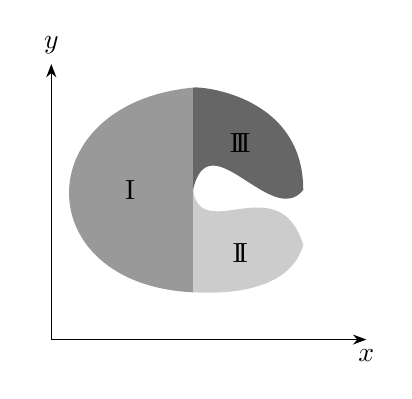
\begin{tikzpicture}
\draw[-Stealth](0,0)--(4,0)node[below]{$x$};
\draw[-Stealth](0,0)--(0,3.5)node[above]{$y$};
\coordinate(a) at (1.8,0.6);
\coordinate(b) at (1.8,3.2);
\coordinate(c) at (3.2,1.9);
\coordinate(d) at (3.2,1.2);
\coordinate(e) at (1.8,1.9);
\fill[black!40](a)..controls(-0.3,0.7)and(-0.3,3.0)..(b)--(a);
\fill[fill=black!60](b)..controls(1.9,3.22)and(3.2,3.1)..(c)..controls(2.8,1.4)and(2,2.8)..(e)--(b);
\fill[fill=black!20](e)..controls(1.9,1.2)and(2.9,2.2)..(d)..controls(3,0.5)and(1.9,0.6)..(a)--(e);
\node at(1,1.9){I};\node at(2.4,1.1){I$\!$I};
\node at(2.4,2.5){I$\!$I$\!$I};
\end{tikzpicture}
\begin{tikzpicture}
\draw[-Stealth](0,0)--(4,0)node[below]{$x$};
\draw[-Stealth](0,0)--(0,3.5)node[above]{$y$};
\node[below left]at(0,0){$O$};
\filldraw[gray!30,rotate=45,draw=black!80](2.8,0)ellipse(1.4 and 1.1);
\node at(2,2){$D$};
\draw[densely dashed](2.3,3.24)-|(0,0);
\draw[densely dashed](1.67,0.72)-|(0,0);
\draw[densely dashed](0.715,1.7)|-(0,0);
\draw[densely dashed](3.24,2.37)|-(0,0);
\node[left]at(0,3.24){$d$};
\node[left]at(0,0.72){$c$};
\node[below]at(0.715,0){$a$};
\node[below]at(3.24,0){$b$};
\end{tikzpicture}
\begin{tikzpicture}
\draw[-Stealth](0,0)--(4,0)node[below]{$x$};
\draw[-Stealth](0,0)--(0,3.5)node[above]{$y$};
\node[below left]at(0,0){$O$};
\coordinate(a) at (0.8,1.3);
\coordinate(b) at (3.5,1.3);
\coordinate(c) at (0.8,2.2);
\coordinate(d) at (3.5,2.4);
\coordinate(e) at (2.9,2.3);
\coordinate(f) at (2,0.8);
\coordinate(g) at (2,2.7);
\filldraw[fill=gray!30,draw=black](a)--(c)..controls(1.3,2.65)..(g)..controls(2.1,2.7)and(2.55,2.6)
..(e)--(d)--(b)..controls(2,0.5)..(a);
\draw(f)--(g);\draw[densely dashed](f)--(2,0)node[below]{$x$};
\draw[densely dashed](2,0.7)--(0,0.7)node[left]{$\varphi_1(x)$};
\draw[densely dashed](g)--(0,2.7)node[left]{$\varphi_2(x)$};
\draw[densely dashed](a)--(0.8,0)node[below]{$a$}(b)--(3.5,0)node[below]{$b$};
\node at(2.7,1.8){$D$};
\end{tikzpicture}
\begin{tikzpicture}
\draw[-Stealth](0,0)node[below]{$O$}--(4,0)node[below]{$A$};
\coordinate(a)at (20:2);\coordinate(b)at(20:4);
\coordinate(c)at (60:2);\coordinate(d)at(60:4);
\coordinate(O)at(0,0);
\draw[densely dashed](O)--(a)(O)--(c);
\filldraw[fill=gray!30,draw=black](a)--(b)arc(20:60:4)--(c)..controls(40:1.6)..(a);
\draw[-{Stealth[width=0pt 6]}](1.1,0)arc(0:20:1.1)node[below right]{$\alpha$};
\draw[-{Stealth[width=0pt 6]}](0.6,0)arc(0:60:0.6)node[right=2.5pt]{$\beta$};
\node at(40:3){$D$};\node at (40:4.2){\rotatebox{-50}{$\rho=\varphi_2(\theta)$}};
\fill[white](60:1.6)circle(6pt);
\node at (50:1.5){\rotatebox{-50}{$\rho=\varphi_1(\theta)$}};
\end{tikzpicture}
\begin{tikzpicture}
\draw[-Stealth](0,0)node[below]{$O$}--(4,0)node[below]{$A$};
\coordinate(a)at (20:3.5);\coordinate(b)at(60:3.5);
\coordinate(O)at(0,0);
\draw[densely dashed](O)--(a)(O)--(b);
\filldraw[fill=gray!30,draw=black](a)..controls(30:4.2)and(50:4.2)..(b)
..controls(50:2.8)and(30:2.8)..(a);
\draw[-{Stealth[width=0pt 6]}](1.1,0)arc(0:20:1.1)node[below right]{$\alpha$};
\draw[-{Stealth[width=0pt 6]}](0.6,0)arc(0:60:0.6)node[right=2.5pt]{$\beta$};
\node at(40:3.4){$D$};\node at (40:4.2){\rotatebox{-50}{$\rho=\varphi_2(\theta)$}};
\node at (40:2.7){\rotatebox{-50}{$\rho=\varphi_1(\theta)$}};
\end{tikzpicture}
\begin{tikzpicture}
\draw[-Stealth](0,0)node[below]{$O$}--(5,0)node[below]{$A$};
\coordinate(a)at (20:2);\coordinate(b)at(20:4);
\coordinate(c)at (60:2);\coordinate(d)at(60:4);
\coordinate(O)at(0,0);
\draw[densely dashed](O)--(a)(O)--(c);
\filldraw[fill=gray!30,draw=black](a)--(b)
..controls(30:4.5)and(50:4.5)..(d)--(c)..controls(40:1.6)..(a);
\draw[-{Stealth[width=0pt 6]}](0.8,0)arc(0:20:0.8)node[below=4pt,right]{$\alpha$};
\draw[-{Stealth[width=0pt 6]}](0.6,0)arc(0:60:0.6)node[right=2.5pt]{$\beta$};
\draw[densely dashed](O)--(40:1.67)node[above]{$E$};
\draw(40:1.67)--(40:4.26)node[above]{$F$};
\node at(50:3){$D$};
\draw[-{Stealth[width=0pt 6]},densely dashed](1.2,0)arc(0:40:1.2)node[right=2.5pt]{$\theta$};
\draw[densely dashed](40:1.66)arc(40:0:1.66)node[below]{$\varphi_1(x)$};
\draw[densely dashed](40:4.26)arc(40:0:4.26)node[below]{$\varphi_2(x)$};
\end{tikzpicture}
\begin{tikzpicture}
\draw[-Stealth](0,0)node[below]{$O$}--(4,0)node[below]{$A$};
\coordinate(a)at (20:3.5);\coordinate(b)at(60:3.5);
\coordinate(O)at(0,0);
\filldraw[fill=gray!30,draw=black](O)--(a)..controls(30:4.2)and(50:4.2)..(b)
--(O);
\draw[-{Stealth[width=0pt 6]}](1.1,0)arc(0:20:1.1)node[below right]{$\alpha$};
\draw[-{Stealth[width=0pt 6]}](0.6,0)arc(0:60:0.6)node[right=2.5pt]{$\beta$};
\node at(40:2.4){$D$};\node at (40:4.2){\rotatebox{-50}{$\rho=\varphi(\theta)$}};
\end{tikzpicture}

\begin{tikzpicture}[
node distance=-1mm,
every node/.style={circle, text width=2cm, align=center, node font=\scriptsize}]%
\node[rectangle, fill=red, minimum height=1cm, opacity=.9, text width=6cm, align=left, outer sep=5mm]
(main) at (0,0) {main layer};
\begin{scope}[on glass layer]
\node[fill=blue!20, above=of main.center] (glass) {glass\\layer};
\end{scope}
\begin{scope}[on background layer={fill=yellow!90!black}]
\fill (main.south west) rectangle (main.north east)
node [rectangle, anchor=north east, minimum size=0pt] {background};
\end{scope}
\begin{scope}[on above layer]
\node[fill=green!80, below right=of main.center] (above) {above\\layer};
\end{scope}
\begin{scope}[on behind layer]
\node[fill=magenta!90, below left=of main.center] (behind) {behind\\layer};
\end{scope}
\end{tikzpicture}
\begin{tikzpicture}
\filldraw[fill=gray!30,draw=black,rotate=-60](0.2,0.15)ellipse(1.7 and 1.3);
\draw[-Stealth](0,0)node[below]{$O$}--(3.2,0)node[below]{$A$};
\node at(60:0.8){$D$};
\node at(47:1.7){\rotatebox{-50}{$\rho=\varphi(\theta)$}};
\end{tikzpicture}
\begin{tikzpicture}%%%作圆的切线
\draw[help lines](0,0)grid(3,2);
\coordinate(a)at(3,2);
\node[circle,draw](c)at(1,1)[minimum size=40pt]{$c$};
\draw[red](a)--(tangent cs:node=c,point={(a)},solution=1)
--(c.center)--(tangent cs:node=c,point={(a)},solution=2)--cycle;
\draw[blue](3,1)--(tangent cs:node=c,point={(3,1)},solution=2);
\end{tikzpicture}

\begin{tikzpicture}
\clip(-2,-2)rectangle(2,2);
\draw[name path=curve1](-2,-1)..controls(8,-1)and(-8,1)..(2,1);
\draw[name path=curve2](-1,-2)..controls(-1,8)and(1,-8)..(1,2);
\fill[name intersections={of=curve1 and curve2,name=i,total=\t}]
[red,opacity=0.5,every node/.style={above left,black,opacity=1}]
\foreach \s in{1,...,\t}{(i-\s)circle(2pt)node{\s}};
\end{tikzpicture}
\begin{tikzpicture}
\clip(-2,-2)rectangle(2,2);
\draw[name path=curve1](-2,-1)..controls(8,-1)and(-8,1)..(2,1);
\draw[name path=curve2](-1,-2)..controls(-1,8)and(1,-8)..(1,2);
\fill[name intersections={of=curve1 and curve2,by={a,b,c}}]
(a) circle (2pt) (b)circle(2pt)(c)circle(3pt);
\end{tikzpicture}
\begin{tikzpicture}%%%%按照路径顺序命名
\clip (-0.5,-0.75) rectangle (3.25,2.25);
\foreach \pathname/\shift in {line/0cm, curve/2cm}{ \tikzset{xshift=\shift}
\draw [-stealth, name path=curve] (1,1.5) .. controls (-1,1) and (2,0.5) .. (0,0); \draw [-latex, name path=line] (0,-.5) -- (1,2) ;
\fill [name intersections={of=line and curve,sort by=\pathname, name=i}] [red, opacity=0.5, every node/.style={left=.25cm, black, opacity=1}]
\foreach \s in {1,2,3}{(i-\s) circle (2pt) node {\footnotesize\s}};
}

\end{tikzpicture}
\tikz \draw (0,0) arc [start angle=70,delta angle=-50, radius=1.5cm] -- ([turn]30:1cm);

\begin{tikzpicture}
\foreach \ang in {0,30,...,90}
\draw [very thick] (0,0) node [below] {(0,0)}-- (\ang:2)
([turn] 0.7,0) node {$\ang^\circ$};
\foreach \ang in {0,30,...,90}
{\draw [very thick] (6,0) node [below] {(6,0)} -- +(\ang:2)
coordinate (d\ang) circle (10pt)
([turn] 0.7,0) node {$\ang^\circ$};
\draw [green] (0,0) -- ($(0,0)!1.2!(d\ang)$);}
\end{tikzpicture}
\tikz \draw[double] plot[smooth cycle] coordinates{(0,0) (1,1) (1,0) (0,1)};%%画双线

\begin{tikzpicture}
\draw[fill=red,pattern=fivepointed stars]
(0,0) circle (1cm);
\draw[pattern=fivepointed stars,fill=cyan]
(0,0) rectangle (2,1);
\end{tikzpicture}
\begin{tikzpicture}
\draw[pattern color=red,pattern=fivepointed stars] (0,0) circle (1cm);
\draw[pattern color=blue,pattern=fivepointed stars] (0,0) rectangle (2,1);
\end{tikzpicture}
\begin{tikzpicture}
\def\mypath{(0,0) -- +(0,1) arc (180:0:1.5cm) -- +(0,-1)} \fill [red] \mypath;
\pattern[pattern color=white,pattern=bricks] \mypath;
\end{tikzpicture}
\tikz\fill [nonzero rule](0,0)circle(1cm)(1,0)circle(1cm);\hspace{2cm}
\tikz\fill [even odd rule](0,0)circle(1cm)(1,0)circle(1cm);

\begin{tikzpicture}
\draw[red] (0,0) circle (4pt);
\draw[red] (2,1) circle (6pt);
\draw (current bounding box.south west) rectangle (current bounding box.north east);
\draw[red] (3,-1) circle (8pt);
\draw[thick] (current bounding box.south west) rectangle (current bounding box.north east);
\end{tikzpicture}
\begin{tikzpicture}[domain=0:4]
\draw[very thin,color=gray] (-0.1,-1.1) grid (3.9,2.8);
\draw[-stealth] (-0.2,0) -- (4.2,0) node[right] {$x$};
\draw[-stealth] (0,-1.2) -- (0,3) node[above] {$f(x)$};
\draw[color=blue] plot (\x,{sin(\x r)}) node[right] {$f(x) = \sin x$};
\draw[color=orange] plot (\x,{0.05*exp(\x)})
node[right] {$f(x) = \frac{1}{20} \mathrm e^x$};
\path [clip] plot (\x,{sin(\x r)});
\fill[pattern=crosshatch] plot (\x,{0.05*exp(\x)})--(0,3)--cycle;
\end{tikzpicture}
\tikz[very thick]{
\tikzmath{\banjing=1.5;}
\fill[fill=gray!30] circle (\banjing);
\fill[fill=white] (-1,1) circle (\banjing);
\fill[fill=white] (1,1) circle (\banjing);
{[]%%%%%%%等效于scope环境
\clip circle (1.5);
\clip (-1,1) circle (\banjing);
\fill [fill=gray!30] (1,1) circle (\banjing);
}
\draw circle (\banjing);
\draw (-1,1) circle (\banjing);
\draw (1,1) circle (\banjing);
}

\tikz\node foreach \x in {1,...,4} foreach \y in{1,2,3}
[draw] at (\x,\y){$\x,\y$};
\begin{tikzpicture}
[every rectangle node/.style={draw},every circle node/.style={draw,double}]
\draw(0,0)node[rectangle]{A}--(1,1)node[circle]{B};
\end{tikzpicture}
\begin{tikzpicture}[every node/.style=draw,
    label/.style={sloped,above,font=\footnotesize},
    every node/.style={rounded corners,draw}]
    \node(content resolver)[fill=blue!30,draw=blue] {ContentResolver};
    \node(android)[fill=orange!50,rounded corners,draw=orange,above right=of content resolver]{Android系统};
    \node(content provider) [fill=blue!30,draw=blue,below right=of android]{ContentProvider};
    \node(file system)[below left=of content provider]{文件系统};
    \node(sqlite)[below=of content provider]{Sqlite数据库};
    \node(network)[below right=of content provider]{网络};
    \node(manifest)[above right=of android,xshift=5mm,yshift=-1cm,fill=red!20]{AndroidManifest.xml};

    \draw(content resolver) edge[out=90,in=180,"URI"draw=none,near end,label] (android);
    \draw(android)edge[out=0,in=100,"URI"draw=none,near start,label](content provider);
    \draw(content provider)edge[-](content resolver);
    \draw(android.north)edge[out=120,in=50,thick,dotted,sloped,font=\footnotesize,"根据URI匹配ContentProvider"'draw=none,-](manifest.east);
    \draw[-](content provider)--(file system)
            (content provider)--(sqlite)
            (content provider)--(network);
\end{tikzpicture}
\begin{tikzpicture}[pin distance=15mm,every pin edge/.style={<-,shorten <=1pt,decorate,decoration={snake,pre length=4pt,segment length=4pt,amplitude=0.5pt}}]
\node[circle,draw,pin=right:X,pin=above right:Y,pin=above:Z,pin=below:U]{circle};
\end{tikzpicture}
\begin{tikzpicture}[smooth cycle,blue]
\node foreach \name/\angle in{a/0,b/90,c/180,d/270}(\name)at(\angle:1.5){$\name$};
\path[-stealth](b) edge node[above right]{$5$}(a)
                  edge(c)
                  edge[-stealth,dotted]node[below,sloped]{missing}(d)
                  (c)edge(a)
                     edge(d)
                  (d)edge[red]node[above,sloped]{very}
                              node[below,sloped]{bad}(a);
\end{tikzpicture}
\tikz[font=\footnotesize,grow=right,level 1/.style={sibling distance=6em},
level 2/.style={sibling distance=1em},level distance=5cm]
  \node{1}
   child{node{1.1}
     child{node{1.1.1}}
     child{node{1.1.2}}
     child{node{1.1.3}}
     child{node{1.1.4}}
  }
   child{node{1.2}
     child{node{1.2.1}}
     child{node{1.2.2}}
     child{node{1.2.3}}
     child{node{1.2.4}}
  }
   child{node{1.3}
     child{node{1.3.1}}
     child{node{1.3.2}}
     child{node{1.3.3}}
     child{node{1.3.4}}
  }
   child{node{1.4}
     child{node{1.4.1}}
     child{node{1.4.2}}
     child{node{1.4.3}}
     child{node{1.4.4}}
     child{node{1.4.5}}
  }
   child{node{1.5}
     child{node{1.5.1}}
     child{node{1.5.2}}
     child{node{1.5.3}}
     child{node{1.5.4}}
     child{node{1.5.5}}
  };
  %[text width=2.7cm,align=flush center,grow cyclic,
%level 1/.style={level distance=2.5cm,sibling angle =75},
%level 2/.style={text width=2cm,font=\footnotesize,level distance=3cm,sibling angle=30}
%]
  \tikz[mindmap,every node/.style=concept,concept color=black!20,grow cyclic,
  level 1/.append style={level distance=4.5cm,sibling angle=72},
  level 2/.append style={level distance=3cm,sibling angle=35}
]
  \node[root concept]{1}
   child{node{1.1}
     child{node{1.1.1}}
     child{node{1.1.2}}
     child{node{1.1.3}}
     child{node{1.1.4}}
  }
   child{node{1.2}
     child{node{1.2.1}}
     child{node{1.2.2}}
     child{node{1.2.3}}
     child{node{1.2.4}}
  }
   child{node{1.3}
     child{node{1.3.1}}
     child{node{1.3.2}}
     child{node{1.3.3}}
     child{node{1.3.4}}
  }
   child{node{1.4}
     child{node{1.4.1}}
     child{node{1.4.2}}
     child{node{1.4.3}}
     child{node{1.4.4}}
     child{node{1.4.5}}
  }
   child{node{1.5}
     child{node{1.5.1}}
     child{node{1.5.2}}
     child{node{1.5.3}}
     child{node{1.5.4}}
     child{node{1.5.5}}
  };

  \begin{tikzpicture}[mindmap]
\begin{scope}[
every node/.style={concept,circular drop shadow,execute at begin node=\hskip0pt},
root concept/.append style={
  concept color=black,fill=white,line width=1ex,text=black,font=\large\scshape},
  text=white,yi/.style={concept color=red,faded/.style={concept color=red!50}},
  er/.style={concept color=blue,faded/.style={concept color=blue!50}},
  san/.style={concept color=orange,faded/.style={concept color=orange!50}},
  si/.style={concept color=green!50!black,faded/.style={concept color=green!50!black!50}},
  wu/.style={concept color=orange,faded/.style={concept color=orange!50}},
  grow cyclic,
  level 1/.append style={level distance=4.5cm,sibling angle=72,font=\scshape},
  level 2/.append style={level distance=3cm,sibling angle=35,font=\scriptsize}
]
  \node[root concept]{1}
   child[yi]{node{1.1}
     child{node{1.1.1}}
     child{node{1.1.2}}
     child[faded]{node{1.1.3}}
     child{node{1.1.4}}
  }
   child[er]{node{1.2}
     child{node{1.2.1}}
     child[faded]{node{1.2.2}}
     child{node{1.2.3}}
     child{node{1.2.4}}
  }
   child[san]{node{1.3}
     child{node{1.3.1}}
     child[faded]{node{1.3.2}}
     child{node{1.3.3}}
     child{node{1.3.4}}
  }
   child[si]{node{1.4}
     child{node{1.4.1}}
     child[faded]{node{1.4.2}}
     child{node{1.4.3}}
     child{node{1.4.4}}
     child[faded]{node{1.4.5}}
  }
   child[wu]{node{1.5}
     child[faded]{node{1.5.1}}
     child{node{1.5.2}}
     child{node{1.5.3}}
     child{node{1.5.4}}
     child[faded]{node{1.5.5}}
  };
\end{scope}
\end{tikzpicture}
%\def\lecture#1#2#3#4#5#6{
%\node[annotation,#3,scale=0.65,text width=4cm,inner sep=2mm,fill=white]at(#4){
%  Lecture #1:\textcolor{orange}{\textbf{#2}}
%  \list{--}{\topsep=2pt\itemsep=0pt\parsep=0pt
%  \parskip=0pt\labelwidth=8pt\leftmargin=8pt
%  \itemindent=0pt\labelsep=2pt}
%  #5
%  \endlist
%  };
%  \node[anchor=base west] at(cal-#6.base east){\textcolor{orange}{\textbf{#2}}};
%  }
%\noindent
%\begin{tikzpicture}
%\begin{scope}[mindmap,
%every node/.style={concept,circular drop shadow,execute at begin node=\hskip0pt},
%root concept/.append style={
%  concept color=black,fill=white,line width=1ex,text=black,font=\large\scshape},
%  text=white,yi/.style={concept color=red,faded/.style={concept color=red!50}},
%  er/.style={concept color=blue,faded/.style={concept color=blue!50}},
%  san/.style={concept color=orange,faded/.style={concept color=orange!50}},
%  si/.style={concept color=green!50!black,faded/.style={concept color=green!50!black!50}},
%  wu/.style={concept color=db,faded/.style={concept color=db!50}},
%  grow cyclic,
%  level 1/.append style={level distance=4.5cm,sibling angle=72,font=\scshape},
%  level 2/.append style={level distance=3cm,sibling angle=35,font=\scriptsize}
%]
%  \node[root concept](CCY){1}
%   child[yi]{node[yshift=-1cm](Computational Problems){1.1}
%     child{node{1.1.1}}
%     child{node{1.1.2}}
%     child[faded]{node{1.1.3}}
%     child{node{1.1.4}}
%  }
%   child[er]{node[yshift=-1cm](Computational Models){1.2}
%     child{node{1.2.1}}
%     child[faded]{node{1.2.2}}
%     child{node{1.2.3}}
%     child{node{1.2.4}}
%  }
%   child[san]{node[yshift=-1cm]{1.3}
%     child{node{1.3.1}}
%     child[faded]{node{1.3.2}}
%     child{node{1.3.3}}
%     child{node{1.3.4}}
%  }
%   child[si]{node[yshift=-1cm]{1.4}
%     child{node{1.4.1}}
%     child[faded]{node{1.4.2}}
%     child{node{1.4.3}}
%     child{node{1.4.4}}
%     child[faded]{node{1.4.5}}
%  }
%   child[wu]{node[yshift=-1cm]{1.5}
%     child[faded]{node{1.5.1}}
%     child{node{1.5.2}}
%     child{node{1.5.3}}
%     child{node{1.5.4}}
%     child[faded]{node{1.5.5}}
%  };
%\end{scope}
%\tiny\calendar[day list downward,
%               month text=\%mt\  \%y0,
%               month yshift=3.5em,
%               name=cal,
%               at={(-.5\textwidth-5mm,.5\textheight-1cm)},
%               dates=2009-04-01 to 2009-06-last]
%  if(weekend)[black!25]
%  if(day of month=1){
%   \node at (0pt,1.5em)[anchor=base west]{\small\tikzmonthtext};
%};
%\lecture{1}{Computational Problems}{above,xshift=-5mm,yshift=5mm}
%{Computational Problems.north}{
%\item Knowledge of several key problems
%\item Knowledge of problem encoding
%\item Being able to formalize problems
%}{2009-04-05}
%\lecture{2}{Computational Models}{above left}
% {Computational Models.west}{
% \item Knowledge of Turing machines
% \item Being able to compare the computational power of different models
% }{2009-04-15}
%\begin{pgfonlayer}{background}
%\clip[xshift=-1cm](-.5\textwidth,-.5\textheight) rectangle ++(\textwidth,\textheight);
%\colorlet{upperleft}{green!50!black!25}
%\colorlet{upperright}{orange!25}
%\colorlet{lowerleft}{red!25}
%\colorlet{lowerright}{blue!25}
%\fill[upperleft](CCY)rectangle ++(-20,20);
%\fill[upperright](CCY)rectangle ++(20,20);
%\fill[lowerleft](CCY)rectangle ++(-20,-20);
%\fill[lowerright](CCY)rectangle ++(20,-20);
%\shade[left color=upperleft,right color=upperright]
%([xshift=-1cm]CCY)rectangle++(2,20);
%\shade[left color=lowerleft,right color=lowerright]
%([xshift=-1cm]CCY)rectangle++(2,-20);
%\shade[top color=upperleft,bottom color=lowerleft]
%([yshift=-1cm]CCY)rectangle++(-20,2);
%\shade[top color=upperright,bottom color=lowerright]
%([yshift=-1cm]CCY)rectangle++(20,2);
%\end{pgfonlayer}
%\end{tikzpicture}
%\tikzstyle{mystyle}{
%->, % makes the edges directed
%>=stealth', % makes the arrow heads bold
%node distance=3cm, % specifies the minimum distance between two nodes. Change if necessary.
%every state/.style={thick, fill=gray!10}, % sets the properties for each 'state' node
%initial text=$ $, % sets the text that appears on the start arrow
%}
%\begin{center}
%  \begin{tikzpicture}[mystyle]
%  \node[state, initial ] (q1) {$q_1$};
%\node[state, right of=q1] (q2) {$q_2$};
%\node[state, right of=q2] (q3) {$q_3$};
%\node[state] at (4.5, 3) (q5) {$q_5$};
%\node[state, accepting] at (0, -3) (q6) {$q_{reject}$};
%\node[state, accepting,right of=q6] (q7) {$q_{accept}$};
%\node[state, right of=q7] (q4) {$q_4$};
%
%\draw (q1) edge[below] node{$0\rightarrow \sqcup,R$}(q2)
%(q2) edge[below] node{$0\rightarrow x,R$}(q3)
%(q5) edge[above,pos=.2, left=2pt] node{$\sqcup\rightarrow R$}(q2)
%(q3) edge[above,pos=.5, right=2pt] node{$\sqcup\rightarrow L$}(q5)
%(q1) edge[above,pos=.5, left=2pt] node{$\sqcup\rightarrow R,x\rightarrow R$}(q6)
%(q2) edge[above,pos=.5, right=2pt] node{$\sqcup\rightarrow R$}(q7)
%%直线部分画完
%(q2) edge[loop,left] node{$x\rightarrow R$}(q2);
%\end{tikzpicture}
%\end{center}

\begin{tikzpicture}
\draw[-Stealth](-3.2,0)--(3.2,0)node[below]{$x$};
\draw[-Stealth](0,-2.2)--(0,2.2)node[left]{$y$};
\draw(-3,-1)--(-2,0)--(-1,-1)--(0,-1);
\draw(0,1)--(3,1);\node at(-1.5,1){$y=f(x)$};
\filldraw[fill=white,draw=black](-2,0)circle(1pt);
\filldraw[fill=white,draw=black](0,-1)circle(1pt);
\filldraw[fill=white,draw=black](0,1)circle(1pt);
\fill[black](0,0)circle(1pt);
\foreach \x in{-2,-1,1}
\node[below]at(\x,0){$\x$};
\node[left]at(0,1){$1$};\node[right]at(0,-1){$-1$};
\foreach \x in{-1,1}
\draw(\x,0)--(\x,1pt);
\end{tikzpicture}
\begin{tikzpicture}
\draw[-Stealth](-1.7,0)--(3.1,0)node[below]{$x$};
\draw[-Stealth](0,-2.2)--(0,2.2)node[left]{$y$};
\draw(-1,-1)--(0,0)--(1,-1);
\draw(1,0)--(2,1);
\node at(1,1){$y=f(x)$};
\filldraw[fill=white,draw=black](0,0)circle(1pt)node[above left]{$O$};
\filldraw[fill=white,draw=black](1,-1)circle(1pt);
\filldraw[fill=white,draw=black](-1,-1)circle(1pt);
\filldraw[fill=white,draw=black](2,1)circle(1pt);
\fill[black](0,1)circle(1pt)node[left]{$1$};
\fill[black](1,0)circle(1pt);
\foreach \x in{-1,1,2}
\node[below]at(\x,0){$\x$};
\foreach \x in{-1,2}
\draw(\x,0)--(\x,1pt);
\draw(0,-1)node[left]{$-1$}--(-1pt,-1);
\end{tikzpicture}
\begin{tikzpicture}
\draw(0,0)node[below]{$O$}--(3,0)node[below]{$A$}arc(0:90:3)--cycle;
\draw(3,0)--node[right=-2pt]{$\tan x$}(3,3)node[right]{$D$}--({3*sin(45)},{3*cos(45)})node[above]{$B$}--node[above]{$1$}
(0,0);
\coordinate(B)at({3*sin(45)},{3*cos(45)});
\node(C)at(B|-0,0){};
\node[below]at(B|-0,0){$C$};\draw(B)--node[left=-2pt]{$\sin x$}({3*sin(45)},0);
\draw[semithick](0,0)--node[below=1.6pt]{$\cos x$}({3*sin(45)},0);
\draw(2.02,0)--(2.02,0.1)--(2.12,0.1);
\draw(0:0.3)arc(0:45:0.3);\node at(18:0.5){$x$};
\end{tikzpicture}

\begin{tikzpicture}[shorten <=2pt,every node/.style={align=center}]
\foreach \x in{1,2,3,4,5}
\fill[black!60](0,\x)circle(5pt)node(a\x){};
\fill[black!20](-2,1.5)circle(5pt)node(b1){};
\fill[black!20](-2,2.5)circle(5pt)node(b2){};
\fill[black!20](-2,3.5)circle(5pt)node(b3){};
\fill[black!20](-2,4.5)circle(5pt)node(b4){};
\fill[black](2,3)circle(5pt)node(c){};
\node(y4)at(-3,4.5){$x_1$};
\node(y3)at(-3,3.5){$\vdots$};
\node(y2)at(-3,2.5){$x_n$};
\node(y1)at(-3,1.5){bias:1};
\node at(-2,6){Input\\layer};
\node at(0,6){Hidden\\layer};
\node at(2,6){Output\\layer};
\node(d)at(3.5,3){$N(x,p)$};
\draw[-stealth](c)--(d);
\foreach \x in{1,2,3,4}
\draw[-{stealth[sep=2pt]}](y\x)--(b\x);
\foreach \x in{1,2,3,4}
{\foreach \y in{1,2,3,4,5}
   {\draw[-{stealth[sep=2pt]}](b\x)--(a\y);
    \draw[-{stealth[sep=4pt]}](a\y)--(c.west);
}
}
\end{tikzpicture}
\begin{tikzpicture}
\draw[-Stealth](-2.3,0)--(4,0)node[below]{$x$};
\draw[-Stealth](0,-1.7)--(0,2.8)node[above left]{$y$};
\node[below left] at(0,0){$O$};
\foreach \x in{1,2,3}
\node[below]at(\x,0){$\x$};
\foreach \x in{1,2}
\node[left]at(0,\x){$\x$};
\node[below left=-3pt]at(-1,0){$-1$};
\node[below left=-3pt]at(0,-1){$-1$};\node at(-1.5,-1){$y=x^2-1$};
\draw(-1,0)arc(180:270:1);\draw(0,0)--(1,2)node[right]{$y=f(x)$}--(2,0);\draw[semithick](2,0)--(3,0);
\foreach \x in{-1,0,2,3}
\filldraw[fill=white,draw=black](\x,0)circle(1pt);
\filldraw[fill=white,draw=black](1,2)circle(1pt);
\filldraw[fill=white,draw=black](0,-1)circle(1pt);
\fill[black](1,1)circle(1pt);\draw(1,0)--(1,1pt)(0,1)--(1pt,1)(0,2)--(1pt,2);
\end{tikzpicture}
\begin{tikzpicture}
\draw[-Stealth](-0.3,0)--(4,0)node[below]{$x$};
\draw[-Stealth](0,-0.3)--(0,3.8)node[left]{$y$};
\node[below left]at(0,0){$O$};
\draw(0.8,0.6)arc(-90:0:2.5)node[left]{$y=f(x)$};
\draw[domain=0.5:3.5]plot(\x,{0.6*\x-0.3})node[right]{$T$};
\draw(0.8,0)arc(0:30.96:0.3cm);
\draw[densely dashed](2,0.9)node[above]{$M$}--(2,0)node[below]{$x_0$};
\node at(0.95,0.13){$\alpha$};
\end{tikzpicture}
\begin{tikzpicture}
\draw[-Stealth](-3,0)--(3,0)node[below]{$x$};
\draw[-Stealth](0,-1.8)--(0,1.8)node[left]{$y$};
\draw[domain=-2.7:2.7,samples=200]plot(\x,{\x^(1/3)})node[above left]{$y=\sqrt[3]x$};
\end{tikzpicture}
\begin{tikzpicture}
\begin{scope}[x={(-0.4cm,-0.4cm)},y={(1cm,0cm)},z={(0cm,1cm)}]
\draw[-Stealth](0,0,0)--(3,0,0)node[anchor=north]{$x$};
\draw[-Stealth](0,0,0)--(0,3,0)node[below]{$y$};
\draw[-Stealth](0,0,0)--(0,0,3)node[left]{$z$};
\draw[-{Stealth[width=0pt 6]}](0,0,0)--(2.5,2,2.5);
\node[left]at(0,0){$O$};
\draw[densely dashed](2.5,2,2.5)--node[right]{$\mathrm dz_i$}(2.5,2,0)--(0,0,0)
(2.5,2,0)--node[below]{$\mathrm dy_i$}(2.5,0,0)(2.5,2,0)--node[right]{$\mathrm dx_i$}(0,2,0);
\end{scope}
\draw[-{Stealth[scale=0.5]}](-0.2,-0.2)arc(-135:-50:0.28);
\node at(0,-0.48){$\theta_i$};
\draw[-{Stealth[scale=0.5]}](-50:0.24)arc(-50:60:0.24);
\node at(0.45,0.1){$\phi_i$};
\end{tikzpicture}
\begin{tikzpicture}
	\node[above,xscale=1.2,yscale=1.4]{\Huge\bfseries 我是祖国花朵,你是什么};
	\node[xscale=1.2,above,yscale=-1.4,scope fading=south,opacity=0.4]{\Huge\bfseries 我是祖国花朵,你是什么};
	\end{tikzpicture}

\begin{tikzpicture}[>=stealth]
\draw[->](0,0,0)--(2,0,0)node[at end,right]{$x$};
\draw[->](0,0,0)--(0,2,0)node[at end,left]{$y$};
\draw[->](0,0,0)--(0,0,2)node[at end,left]{$z$};
\draw[red,rotate around x=0](0,0,0)--(1,1,0)--(1,0,0);
\draw[blue,rotate around x=45](0,0,0)--(1,1,0)--(1,0,0);
\draw[green,rotate around x=90](0,0,0)--(1,1,0)--(1,0,0);
\draw[green!50,rotate around y=-90](0,0,0)--(1,1,0)--(1,0,0);
\draw[green!50,rotate around z=45](0,0,0)--(1,1,0)--(1,0,0);
\end{tikzpicture}
\begin{tikzpicture}[z={(10:10mm)},x={(-45:5mm)}]
\def\wave{
  \draw[fill,thick,fill opacity=0.2]
  (0,0)sin(1,1)cos(2,0)sin(3,-1)cos(4,0)
  sin(5,1)cos(6,0)sin(7,-1)cos(8,0)sin(9,1)cos(10,0)sin(11,-1)cos(12,0);
  \foreach \shift in{0,4,8}
  {
  \begin{scope}[xshift=\shift cm,thin]
  \draw(.5,0)--(0.5,0|-45:1cm);
  \draw(1,0)--(1,1);
  \draw(1.5,0)--(1.5,0|-45:1cm);
  \draw(2.5,0)--(2.5,0|--45:1cm);
  \draw(3,0)--(3,-1);
  \draw(3.5,0)--(3.5,0|--45:1cm);
  \end{scope}
  }
  }
 \begin{scope}[canvas is zy plane at x=0,fill=blue]
 \wave
 \node at(6,-1.5)[transform shape]{magenetic field};
 \end{scope}
 \begin{scope}[canvas is zx plane at y=0,fill=red]
   \draw[help lines](0,-2)grid(12,2);
   \wave
   \node at (6,1.5)[rotate=180,xscale=-1,transform shape]{electric field};
 \end{scope}
\end{tikzpicture}
\begin{tikzpicture}
\begin{scope}[canvas is zy plane at x=0]
\draw(0,0)circle(1cm);
\draw(-1,0)--(1,0)(0,-1)--(0,1);
\end{scope}
\begin{scope}[canvas is xz plane at y=0]
\draw(0,0)circle(1cm);
\draw(-1,0)--(1,0)(0,-1)--(0,1);
\end{scope}
\begin{scope}[canvas is yx plane at z=0]
\draw(0,0)circle(1cm);
\draw(-1,0)--(1,0)(0,-1)--(0,1);
\draw[-stealth](-1.1,0)--(1.1,0)node[at end]{$x$};
\draw[-stealth](0,-1.1)--(0,1.1)node[at end]{$y$};
\end{scope}
\end{tikzpicture}
\begin{tikzpicture}
\draw(2,0)coordinate(A)--(0,0)coordinate(B)--(-1,-1)coordinate(C)
pic[fill=gray!30]{angle=A--B--C}
pic[draw,-Stealth,angle radius=0.5cm]{right angle=C--B--A};
\end{tikzpicture}
\begin{tikzpicture}[shorten >=1pt,node distance=2cm,on grid,>=stealth,thick,
every state/.style={fill,draw=none,orange,text=white,circular drop shadow},
accepting/.style={green!50!black,text=white},
initial/.style={red,text=white}
]
\node[state,initial](q_0)                     {$q_0$};
\node[state]        (q_1)[above right=of q_0] {$q_1$};
\node[state]        (q_2)[below right=of q_0] {$q_2$};
\node[state,accepting]        (q_3)[above right=of q_2] {$q_3$};
\path[->](q_0)edge node[above left] {$0$}(q_1)
              edge node[below left] {$1$}(q_2)
         (q_1)edge node[above right]{$1$}(q_3)
              edge[loop above]node  {$0$}()
         (q_2)edge node[below right]{$0$}(q_3)
              edge[loop below]node  {$1$}();
\end{tikzpicture}
\begin{tikzpicture}[->,shorten >=1pt,auto,node distance=2cm,on grid,>=stealth,semithick,
inner sep=2pt,bend angle=45,initial text=开始,accepting by double
]
\node[initial,state](A)                     {$q_a$};
\node[state]        (B)[above right=of A] {$q_b$};
\node[state]        (D)[below right=of A] {$q_d$};
\node[state]        (C)[below right=of B] {$q_c$};
\node[state,accepting]        (E)[below=of D] {$q_e$};
\path[every node/.style={font=\footnotesize}]
         (A)edge node {0,1,L}(B)
              edge node {1,1,R}(C)
         (B)edge[loop above]node{1,1,L}(B)
              edge node  {0,1,L}(C)
         (C)edge node{0,1,L}(D)
         edge[bend left]node{1,0,R}(E)
         (D)edge[loop below]node{1,1,R}(D)
            edge node{1,1,R}(A)
         (E)edge[bend left]node{1,0,R}(A);
\end{tikzpicture}

\begin{tikzpicture}[mindmap,concept color=blue!80,every annotation/.style={fill=red!20,draw=blue!50,minimum height=3cm,font=\zihao{3}}]
\node[concept](root){Root};
\node[annotation,right]at(root.east)
{annotation};
\node[draw,circle](draw)at (0,-4){draw};
\node[annotation,right]at(draw.east){Time forward};
\end{tikzpicture}
\begin{tikzpicture}
\node[scale=0.5,cloud,draw,fill=gray!20,aspect=4,cloud puffs=20]{明天我要参加新东方科大宣讲会};
\node[cloud callout,draw,fill=gray!20,cloud puff arc=120,shading=ball,aspect=2,ball color=gray!30]at(3.5,0){Eddddd};
\node[double arrow,draw]at (0,-3){left or right};
\node[thick,starburst,draw,fill=yellow,draw=red]at(3.5,-3){\bf Boom Shakalaka!};
\end{tikzpicture}

\begin{tikzpicture}[scale=0.8]
\draw[-Stealth](0,0)--(7.2,0)node[below]{$x$};
\draw[-Stealth](0,0)--(0,3)node[left]{$y$};
\node[below left]at(0,0){$O$};
\draw[domain=0:8,samples=200]plot({\x-sin(\x r)},{1-cos(\x r)});
\node[below]at(6.28,0){$2\pi a$};
\draw[densely dashed](0,2)--(7.2,2);
\draw[densely dash dot](-0.3,1)--(7.2,1)(3.1415,0)--(3.1415,2.3)(0.83,-0.2)--(0.83,2.17);
\node[below=2pt]at(3.1415,0){$\pi a$};
\draw (0.83,1)circle(1cm);
\draw[-{Stealth[width=0pt 5]}](0.83,1)--(0.3,1.87);
\node at (0.4,1.4){$a$};
\draw[-{Stealth[width=0pt 5]}](0.83,1)--(0.1,0.32);
\node at(-0.8,0.32){$M(x,y)$};
\fill(0.1,0.32)circle(1pt);
\draw[-{Stealth[width=0pt 6]}](0.83,0.4)arc(-90:-138:0.6);
\node at(0.7,0.64){$t$};
\end{tikzpicture}
\tikzset{
every picture/.style={
>=latex,
node distance=5mm and 5mm
%有无and的区别见手册positioning部分
}}

%定义框形状
\tikzstyle{SS}      %开始结束
=[rounded corners, draw]
\tikzstyle{IO}      %输入输出
=[trapezium, trapezium left angle=70, trapezium right angle=110, draw]
\tikzstyle{NR}      %内容
=[draw]
\tikzstyle{PD}      %判断
=[diamond, aspect=4, draw, inner sep=1.5pt]
\begin{tikzpicture}[->]
\node[draw,rounded corners,minimum width=1.3cm,minimum height=0.6cm](start){开始};
\node[IO, below=of start](in){输入$x$, $t$};
\node[NR, below=of in](n1){$M=1$, $S=3$, $k=1$};
\node[PD, below=of n1](pd){$k\le t$};
\node[NR, on grid, below left=1cm and 2cm of pd](n3){$M=\dfrac Mkx$};
\node[IO, on grid, below right=1cm and 2cm of pd](out){输出$S$};
\node[NR, below=of n3](n4){$S=M+S$};
\node[NR, below=of n4](n5){$k=k+1$};
\node[SS, below=of out](stop){结束};
\path (start) edge (in)
(in) edge (n1)
(n1) edge (pd)
(n3) edge (n4)
(n4) edge (n5)
(out) edge (stop);
\draw (pd) -| node[left]{是} (n3);
\draw (pd) -| node[right]{否} (out);
\draw (n5.west)--++(-0.5,0) |- ($(n1.south)!0.5!(pd.north)$);
\end{tikzpicture}
\begin{tikzpicture}[decoration={brace,amplitude=3pt}]
\coordinate[label=below left:$A$](A)at(0,0);
\coordinate[label=right:$B$](B)at(3,1);
\coordinate[label=above:$C$](C)at(1,4);
\coordinate[label=above right:$A'$](A')at($(B)!0.5!(C)$);
\coordinate[label=above left:$B'$](B')at($(A)!0.5!(C)$);
\coordinate[label=below:$C'$](C')at($(A)!0.5!(B)$);
\draw(A)--(B)--(C)--cycle;
\draw(A)--(A')(B)--(B')(C)--(C');
\coordinate(D)at(intersection of A--A' and C--C')node[above right=-5pt and 0pt of D]{$D$};
\draw[decorate](B)--(A);
\end{tikzpicture}
\begin{tikzpicture}[decoration={brace,amplitude=3pt},opacity=0.5,transparency group]
\begin{scope}[blend mode=screen]
\filldraw[fill=red](0:1cm)circle(12mm);
\filldraw[fill=green](120:1cm)circle(12mm);
\filldraw[fill=blue](-120:1cm)circle(12mm);
\end{scope}
\end{tikzpicture}

\begin{tikzpicture}[scale=0.4,auto,decision/.style={diamond,draw=blue,thick,fill=blue!20,
                   text width=4.5em,align=flush center,inner sep=1pt},
                   block/.style={rectangle,draw=blue,thick,fill=blue!20,
                   text width=5em,align=center,rounded corners,minimum height=4em},
                   line/.style={draw,thick,-latex',shorten >=2pt},
                   cloud/.style={draw=red,thick,ellipse,fill=red!20,minimum height=2em}]
\matrix[column sep=4mm,row sep=7mm]
{\node[cloud](expert){expert};&
\node[block](init){initialize model};&
\node[cloud](system){system};\\
&\node[block](identify){identify candidate model};&\\
\node[block](update){update model};&
\node[block](evaluate){evaluate candidate models};&\\
&\node[decision](decide){is best candidate};&\\
&\node[block](stop){stop};&\\
};
\begin{scope}[every path/.style=line]
\path          (init)--(identify);
\path          (identify)--(evaluate);
\path          (evaluate)--(decide);
\path          (update)|-(identify);
\path          (decide)-|node[near start]{yes}(update);
\path          (decide)--(stop);
\path[dashed]  (expert)--(init);
\path[dashed]  (system)--(init);
\path[dashed]  (system)|-(evaluate);
\end{scope}

\end{tikzpicture}

\begin{tikzpicture}
\begin{scope}[color=Maroon]
\draw[help lines](-7,-7)grid(7,7);
\node[minimum size=14cm](current page1){};
\node[anchor=north west] at (current page1.north west)
{\pgfornament[width=5cm]{35}};
\node[anchor=north east] at (current page1.north east)
{\pgfornament[width=5cm]{36}};
\node[anchor=south west] at (current page1.south west)
{\pgfornament[width=5cm,symmetry=h]{35}};
\node[anchor=south east] at (current page1.south east)
{\pgfornament[width=5cm,symmetry=h]{36}};
\node[scale=2.5,green!45!black,cloud,cloud puffs=14,draw=red]at(current page1.center){\parbox{4cm}{$\displaystyle\int_{-\infty}^{+\infty}{\text{e}^{-x^2}\sin \left( \frac{\pi }{2x^2} \right) \text{d}x}$\\$=\sqrt{\pi}\text{e}^{-\sqrt{\pi}}\sin \left( \sqrt{\pi} \right)$}};
\end{scope}

\end{tikzpicture}
\begin{tikzpicture}[>=Stealth]
\draw[->](0,0)node[below left]{$O$}--(4,0)node[below=2pt]{$x$};
\draw[->](0,0)--(0,3)node[left]{$y$};
\draw(0.5,0.7)..controls(1.3,3.5)and(2.5,0.1)..(3.7,2.4);
\draw(0.5,0.7)node[left]{$A$}--(3.7,2.4)node[right]{$B$};
\draw[domain=0.4:1.6]plot(\x,{0.54*\x+1.2});
\draw[densely dashed](1.1,1.8)node[above]{$C$}--(1.1,0)node[below]{$\xi$};
\draw(1.7,1.82)--(1.7,1.33);\draw(1.7,1.33)--(1.7,0)node[below=2pt]{$x$};
\node at(1.86,1.26){$N$};\node at(1.82,2){$M$};
\draw[densely dashed](0.5,0.7)--(0.5,0)node[below=2pt]{$a$};
\draw[densely dashed](3.7,2.4)--(3.7,0)node[below]{$b$};
\fill(0.5,0.7)circle(0.7pt);
\fill(3.7,2.4)circle(0.7pt);
\fill(1.1,1.79)circle(0.7pt);
\fill(1.7,1.82)circle(0.7pt);
\fill(1.7,1.34)circle(0.7pt);
\end{tikzpicture}
\begin{tikzpicture}[scale=0.9]
\draw
  (-3.5,0) arc (180:0:3.5 and 1.2)
  (-2.5,0) arc (180:0:2.5 and 0.6);
\filldraw[fill = lightgray]
  (0,0) ellipse (2.5 and 0.6);
\filldraw[fill = white]
  (-1.5,-1.5) -- (-1.5,1.5) -- (0,1.0) -- (0,-2.0) -- (-1.5,-1.5)
  -- (-1.5,1.5) -- (0,2.0) -- (1.5,1.5) -- (0,1.0) -- (-1.5,1.5)
  -- (-1.5,-1.5)  -- (0,-2.0) -- (1.5,-1.5) -- (1.5,1.5) -- (0,1.0) -- (0,-2.0);
\fill[fill = lightgray]
  (-1.55,0) rectangle (1.55,-0.6);
\filldraw[fill = white, dashed]
  (-3.5,0) arc (-180:0:3.5 and 1.2)
  (2.5,0) arc (0:-180:2.5 and 0.6)
%  (-1.5,0.1) arc (-180:0:1.5 and 0.6);
  (-1.5,0.0) -- (0.0,-0.5) -- (1.5,0.0);
\draw
  (0.0,0.0) -- (0.0,-0.5)
  (-2.5,0) arc (0:180:0.5 and 0.3)
  (2.5,0) arc (180:0:0.5 and 0.3)
  (-3.5,0) arc (-180:0:3.5 and 1.2)
  (2.5,0) arc (0:-180:2.5 and 0.6);
\draw[dotted]
  (-3.5,0) arc (180:0:3.5 and 1.2)
  (-2.5,0) arc (180:0:2.5 and 0.6)
  (-1.5, -1.5) -- (0,-1.0) -- (1.5,-1.5)
  (0,2.0) -- (0,-1.0)
  (-1.5,0) -- (-1.5,-1.2)
  (1.5,0) -- (1.5,-1.2)
  (-2.5,0) arc (0:-180:0.5 and 0.3)
  (2.5,0) arc (-180:0:0.5 and 0.3);
\draw[dashed]
  (-7,-4) rectangle (6,4)
  (-7,-4) -- (-4.5,-2.5) -- (8,-2.5) -- (6,-4)
  (6,4) -- (8,5.5) -- (8,-2.5)
  (-7,4) -- (-4.5,5.5) -- (-4.5,-2.5)
  (-4.5,5.5) -- (8,5.5);
\node (A) at (4., 2.) {$ \psi,{H}_s $};
\node (B) at (0, 0.2) {$ {T},\psi,u, {H}_s $};
\node (C) at (0.8, -0.85) {${T},\psi,u, {H}_s$};
%\node (C) at (2.0, -0.675) {$ {T},\psi,u $};
\node (D) at (-3,3) {$ \mathcal{S} $};
\draw[dashed]
  (-2,0) -- (D);
\end{tikzpicture}
\begin{tikzpicture}
\draw[-Stealth](0,0)node[below left]{$O$}--(4,0)node[below=1pt]{$x$};
\draw[-Stealth](0,0)--(0,4)node[left]{$y$};
\draw[rotate around={180:(2,2.675)},yshift=0.5cm](0.4,3.8)..controls(2,1.5)..(3.7,3);
\draw[densely dashed](1,2.45)node[left](A){$f(x_1)$}--(1,0)node[below=1pt]{$x_1$};
\draw[densely dashed](3,1.9)node[right](B){$f(x_2)$}--(3,0)node[below=1pt]{$x_2$};
\fill($(A)!0.5!(B)$)circle(0.5pt)node[below=1.7pt,fill=white](C){$\frac{f(x_1)+f(x_2)}2$};
\draw(1,2.45)--(3,1.9);
\fill(1,2.45)circle(0.5pt)(3,1.9)circle(0.5pt)(2,2.87)circle(0.5pt);
\draw[densely dashed](2,2.87)--(2,2.1)(2,1.4)--(2,0)node[below]{$\frac{x_1+x_2}2$};
\node[fill=white] at(2,3.2){$f\left(\frac{x_1+x_2}2\right)$};
\draw[rotate around={180:(2,2.675)},yshift=0.5cm](0.4,3.8)..controls(2,1.5)..(3.7,3);
\fill(2,2.87)circle(0.5pt);
\end{tikzpicture}
\begin{tikzpicture}
\draw[-Stealth](0,0)node[below left]{$O$}--(4,0)node[below=1pt]{$x$};
\draw[-Stealth](0,0)--(0,4)node[left]{$y$};
\draw(0.4,3.8)..controls(2,1.5)..(3.7,3);
\draw[densely dashed](1,2.95)node[left](A){$f(x_1)$}--(1,0)node[below=1pt]{$x_1$};
\draw[densely dashed](3,2.4)node[right](B){$f(x_2)$}--(3,0)node[below=1pt]{$x_2$};
\fill($(A)!0.5!(B)$)circle(0.5pt)node[above](C){$\frac{f(x_1)+f(x_2)}2$};
\draw(1,2.95)--(3,2.4);
\fill(1,2.95)circle(0.5pt)(3,2.4)circle(0.5pt)(2,1.975)circle(0.5pt);
\draw[densely dashed](C)--(2,0)node[below]{$\frac{x_1+x_2}2$};
\node[fill=white] at(2,1.6){$f\left(\frac{x_1+x_2}2\right)$};
\end{tikzpicture}
\begin{tikzpicture}
\draw[-Stealth](-3,0)--(3,0)node[below=1pt]{$x$};
\draw[-Stealth](0,-1)--(0,3)node[left]{$y$};
\node[below left]at(0,0){$O$};
\draw(-2.8,2.6)..controls(-2,-1)and(-1,-1.5)..(-0.1,2);
\draw(0.1,-0.6)..controls(0.6,2)and(2,2.4)..(2.7,2.3)node[above left]{$y=f(x)$};
\end{tikzpicture}

\begin{tikzpicture}
\draw[-Stealth](0,0)--(4,0)node[below=1pt]{$x$};
\draw[-Stealth](0,0)--(0,3.8)node[left]{$y$};
\node[below left]at(0,0){$O$};
\draw(0.4,0.4)arc(-90:0:3)node[above]{$C$};
\fill(0.5,0.404)circle(0.5pt)node[above]{$M_0$}
(1.8,0.747)circle(0.5pt)node[above]{$M$}
(2.9,1.735)circle(0.5pt)node[left=-2pt]{$M'$};
\node at(1.18,0.62){$s$};\node at(2.25,1.35){$\Delta s$};
\draw[-Stealth](0.3,0)--(3.8,1.73);
\draw(0.6,0)arc(0:26.54:0.3);
\node at(0.75,0.1){$\alpha$};
\draw[-Stealth](1.7,0)--(3.8,3.02);
\draw(2,0)arc(0:55.6:0.3);
\node at(2.66,0.15){$\alpha+\Delta\alpha$};
\draw(2.7,1.2)arc(26.54:55.6:0.3);
\node[rotate=26.54]at(2.95,1.47){$\Delta\alpha$};
\end{tikzpicture}
\begin{tikzpicture}
\draw[-Stealth](0,0)--(4,0)node[below=1pt]{$x$};
\draw[-Stealth](0,0)--(0,3.8)node[left]{$y$};
\node[below left]at(0,0){$O$};
\draw(0,0.3)..node[above,sloped,near start]{$y=f(x)$}controls(1,0.3)and(2.7,1.4)..(3.4,2.8);
\draw(2,2.6)coordinate(D)node[left]{$D$}circle(1.053);
\node[below] at (2.8,1.9){$M$};
\coordinate(M)at (2.8,1.9);
\draw(0.9,0)node(B){}--(3.8,2.9);
\draw(D)--(M);
\draw pic[draw,angle radius=0.1cm]{right angle=D--M--B};
\fill(D)circle(0.5pt)node[right=-2pt]{$\rho=\frac1K$}(M)circle(0.5pt);
\end{tikzpicture}
\begin{tikzpicture}
\draw[-Stealth](0,0)node[below left]{$O$}--(4,0)node[below]{$x$};
\draw[-Stealth](0,0)--(0,1.3)node[left]{$y$};
\filldraw[fill=gray!30,draw=black,domain=0:pi](0,0)plot(\x,{sin(\x r)})--cycle;
\node at(1.6,1.2){$y=\sin x$};\node[below]at(3.14,0){$\pi$};
\end{tikzpicture}
\begin{tikzpicture}[samples=100]
\filldraw[samples=100,domain=-1.5:2,fill=gray!30,draw=black,fill=gray!30](-1.5,0)node[below]{$a$}
--(-1.5,0.3077)--plot(\x,{1/(1+(\x)^2)})
--(2,0)node[below]{$b$}--cycle;
\draw[-Stealth](-2.5,0)--(3,0)node[below]{$x$};
\draw[-Stealth](0,-0.5)--(0,1.6)node[left]{$y$};
\node[below left]at(0,0){$O$};
\draw[samples=100,domain=-2:2.4]plot(\x,{1/(1+(\x)^2)})node[above]{$y=\frac1{1+x^2}$};
\end{tikzpicture}

\begin{tikzpicture}[Maroon,scale=0.5]
        \node[text width=8cm,align=center](Text){%
        In visions of the dark night\\
        I have dreamed of joy departed-\\
        But a waking dream of life and light\
        Hath left me broken-hearted.\\

        Ah! what is not a dream by day\\
        To him whose eyes are cast \\
        On things around him with a ray \\
        Turned back upon the past? \\

        That holy dream- that holy dream,\\
        While all the world were chiding,\\
        Hath cheered me as a lovely beam\\
        A lonely spirit guiding.\\

        What though that light, thro' storm and night,\\
        So trembled from afar- \\
        What could there be more purely bright \\
        In Truth's day-star? \\
        \vspace{24pt}
         A Dream (1827) by Edgar Allan Poe
        } ;

        \node[inner sep=0pt,shift={(-.5cm,.5cm)},anchor=north west](CNW)  at (Text.north west)
             {\pgfornament[width=1.75cm]{61}};
        \node[inner sep=0pt,shift={(.5cm,.5cm)},anchor=north east](CNE)   at (Text.north east)
             {\pgfornament[width=1.75cm,symmetry=v]{61}};
        \node[inner sep=0pt,shift={(-.5cm,-.5cm)},anchor=south west](CSW) at (Text.south west)
             {\pgfornament[width=1.75cm,symmetry=h]{61}};
        \node[inner sep=0pt,shift={(.5cm,-.5cm)},anchor=south east](CSE)  at (Text.south east)
             {\pgfornament[width=1.75cm,symmetry=c]{61}};
        \pgfornamenthline{CNW}{CNE}{north}{87}
        \pgfornamenthline{CSW}{CSE}{south}{87}
        \pgfornamentvline{CNW}{CSW}{west}{87}
        \pgfornamentvline{CNE}{CSE}{east}{87}
        \end{tikzpicture}
\newlength\framesize
\framesize=16cm
\begin{tikzpicture}[color=Maroon,
                   transform shape,
                   every node/.style={inner sep=0pt}]
\node[minimum size=\framesize,fill=yellow!20](vecbox){};
\node[anchor=north west] at (vecbox.north west){%
      \pgfornament[width=0.2*\framesize]{63}};
\node[anchor=north east] at (vecbox.north east){%
                         \pgfornament[width=0.2*\framesize,symmetry=v]{63}};
\node[anchor=south west] at (vecbox.south west){%
      \pgfornament[width=0.2*\framesize,symmetry=h]{63}};
\node[anchor=south east] at (vecbox.south east){%
      \pgfornament[width=0.2*\framesize,symmetry=c]{63}};
\node[anchor=north] at (vecbox.north){%
      \pgfornament[width=0.6*\framesize,symmetry=h]{46}};
\node[anchor=south] at (vecbox.south){%
      \pgfornament[width=0.6*\framesize]{46}};
\node[anchor=north,rotate=90]  at (vecbox.west){%
      \pgfornament[width=0.6*\framesize,symmetry=h]{46}};
\node[anchor=north,rotate=-90] at (vecbox.east){%
      \pgfornament[width=0.6*\framesize,symmetry=h]{46}};
\node[inner sep=6pt] (text) at (vecbox.center){\Huge Ornaments};
\node[anchor=north] at (text.south){%
      \pgfornament[width=0.5*\framesize]{75}};
\node[anchor=south] at (text.north){%
      \pgfornament[width=0.5*\framesize,symmetry=h]{75}};
\end{tikzpicture}

\begin{tikzpicture}[scale=1.3]
\draw[-Stealth](0,0)node[below left]{$O$}--(2.5,0)node[below]{$x$};
\draw[-Stealth](0,0)--(0,2)node[left]{$y$};
\filldraw[samples=100,domain=0:1.8,fill=gray!30,draw=black](0,0)--(0,0.5)node[left]{$\frac1a$}--plot(\x,{1/sqrt(4-(\x)^2)})--(1.8,1.149)
--(1.8,0)node[below=-1pt]{$t$}--cycle;
\draw[samples=100,domain=0:1.925]plot(\x,{1/sqrt(4-(\x)^2)});
\node at(0.95,1.2){$y=\frac1{\sqrt{a^2-x^2}}$};
\draw(2,2)--(2,0)node[below]{$a$};
\end{tikzpicture}
\begin{tikzpicture}
\draw[-stealth](0,0)node[below left]{$O$}--(7,0)node[below]{$x$};
\draw[-stealth](0,0)--(0,7)node[left]{$y$};
\filldraw[fill=gray!10](0,0)--(0,pi)node[left]{$\pi$}--(pi,2*pi)--(2*pi,2*pi)--cycle;
\filldraw[fill=gray!20](0,0)--(pi,0)node[below]{$\pi$}--(2*pi,pi)--(2*pi,2*pi)--cycle;
\filldraw[fill=gray!20](0,pi)--(0,2*pi)node[left]{$2\pi$}--(pi,2*pi)--cycle;
\filldraw[fill=gray!10](pi,0)--(2*pi,0)node[below]{$2\pi$}--(2*pi,pi)--cycle;
\node at(pi/4,7*pi/4){正};
\node at(3*pi/4,5*pi/4){负};
\node at(7*pi/4,pi/4){负};
\node at(5*pi/4,3*pi/4){正};
\end{tikzpicture}
\begin{tikzpicture}
\draw[-Stealth](0,0)node[below left]{$O$}--(4,0)node[below=2pt]{$x$};
\draw[-Stealth](0,0)--(0,4)node[left]{$y$};
\draw(.5,0)node[below=2pt]{$a$}--(0.5,1.8)..controls(1.4,3.3)and(2.7,3.6)..(3.6,3.4)
--(3.6,0)node[below]{$b$};
\node at(2.4,3.7){$y=f(x)$};
\filldraw[fill=gray!30](1.5,0)node[below=2pt]{$x$}--node[left=-1pt]{$f(x)$}(1.5,2.91)
--(2,2.91)--(2,0)--cycle;
\node[below=-0.3pt]at(2.3,0){$x+\mathrm dx$};
\node at(1.77,2){$\mathrm dU$};
\end{tikzpicture}
\begin{tikzpicture}[scale=1.5]
\draw[-Stealth](0,0)node[below left]{$O$}--(4,0)node[below=2pt]{$x$};
\draw[-Stealth](0,0)--(0,4)node[left]{$y$};
\draw(.5,0)node[below=2pt]{$a$}--(0.5,1.8)..controls(1.4,3.3)and(2.7,3.6)..(3.5,3.7)
--(3.5,0)node[below]{$b$};
\node at(2.4,3.83){$y=f(x)$};
\draw(.5,0)--(.5,2.05)--(.8,2.05)--(0.8,0)node[below=2pt]{$x_1$}--cycle;
\draw(.8,0)--(.8,2.44)--(1.1,2.44)--(1.1,0)node[below=2pt]{$x_2$}--cycle;
\draw(1.1,0)--(1.1,2.74)--(1.4,2.74)--(1.4,0)--cycle;
\draw(1.4,0)--(1.4,2.98)--(1.7,2.98)--(1.7,0)--cycle;
\draw(1.7,0)--(1.7,3.169)--(2,3.169)--(2,0)node[below=2pt]{$x_{i-1}$}--cycle;
\draw(2,0)--(2,3.34)--(2.3,3.34)--(2.3,0)node[below=2pt]{$x_i$}--cycle;
\draw(2.3,0)--(2.3,3.45)--(2.6,3.45)--(2.6,0)--cycle;
\draw(2.6,0)--(2.6,3.55)--(2.9,3.55)--(2.9,0)--cycle;
\draw(2.9,0)--(2.9,3.625)--(3.2,3.625)--(3.2,0)node[below=2pt]{$x_{n-1}$}--cycle;
\draw(3.2,0)--(3.2,3.68)--(3.5,3.68)--(3.5,0)--cycle;
\draw[densely dashed](0.655,2.05)--(0.655,0.42)node[below]{$\xi_1$};
\draw[densely dashed](0.958,2.44)--(0.958,0.42)node[below]{$\xi_2$};
\draw[densely dashed](2.158,3.34)--(2.158,0.42)node[below]{$\xi_i$};
\draw[densely dashed](3.35,3.68)--(3.35,0.42)node[below]{$\xi_n$};
\end{tikzpicture}
\begin{tikzpicture}[scale=4]
\draw[-Stealth](0,0)node[below left]{$O$}--(1.3,0)node[below]{$x$};
\draw[-Stealth](0,0)--(0,1.3)node[left]{$y$};
\filldraw[fill=gray!30,domain=0:1](0,0)--plot(\x,{(\x)^2})--cycle;
\filldraw[fill=gray!30,domain=0:1](0,0)--plot({(\x)^2},\x)--cycle;
\draw[gray!30,thick](0,0)--(1,1);
\draw[domain=0:1.08](0,0)--plot(\x,{(\x)^2});
\draw[domain=0:1.08](0,0)--plot({(\x)^2},\x);
\node at(0.8,0.4){$y=x^2$};
\node at(0.4,0.8){$y^2=x$};
\draw[densely dashed](1,1)--(1,0)node[below]{$1$};
\draw[densely dashed](1,1)--(0,1)node[left]{$1$};
\node at(1.12,0.96){$(1,1)$};
\end{tikzpicture}

\begin{tikzpicture}
\node[below left]at(0,0){$O$};
\draw[-Stealth,line width=0.4pt](-0.5,0)--(3.5,0)node[below=2pt]{$x$};
\draw[-Stealth,line width=0.4pt](0,-0.5)--(0,2.5)node[above]{$y$};
\node(a)at(1,0.3){};\node(b)at(0.9,2.1){};
\node(c)at(2.2,0.3){};\node(d)at(2,2.1){};
\filldraw[fill=gray!30](a.center)..controls(0.5,0.8)and(1.4,1.5)..(b.center)--(d.center)
..controls(2.7,1.3)and(2.4,0.8)..(c.center)--(a.center);
\draw[densely dashed](1,0.3)--(0,0.3)node[left]{$c$}(0.9,2.1)--(0,2.1)node[left]{$d$};
\node[rotate=-90]at(0.6,1.2){$x=\psi_1(y)$};
\node[rotate=-90]at(2.7,1.2){$x=\psi_2(y)$};
\end{tikzpicture}
\begin{tikzpicture}[color=blue!50]
\draw[help lines](-7,-7)grid(7,7);
\node[minimum size=14cm](mybox){};
\node[anchor=north west] at (mybox.north west){\pgfornament[width=5cm]{63}};
\node[anchor=north east] at (mybox.north east){\pgfornament[width=5cm]{64}};
\node[anchor=south west] at (mybox.south west){\pgfornament[width=5cm,symmetry=h]{63}};
\node[anchor=south east] at (mybox.south east){\pgfornament[width=5cm,symmetry=h]{64}};
\begin{scope}[every node={anchor=center,inner sep=0pt}]
\node[scale=1.8,green!45!black,regular polygon,regular polygon sides=6,rotate=30,minimum size=6cm,inner sep=0pt](s){};
\path(s.side 1)to[ornament=84,color=red](s.side 2)
               to[ornament=84](s.side 3)
               to[ornament=84](s.side 4)
               to[ornament=84](s.side 5)
               to[ornament=84](s.side 6)
               to[ornament=84](s.side 1);
\node[scale=1.8,green!45!black,cloud,cloud puffs=14,draw=red,align=flush center,line width=2pt,text width=2cm]at(mybox.center){\heartpar{Someday, one will find that career, kinship and friendship are more indispensable than romance.}};

\end{scope}
\end{tikzpicture}
\begin{tikzpicture}[scale=4]
\draw[-Stealth](0,0)node[below left]{$O$}--(1.3,0)node[below]{$x$};
\draw[-Stealth](0,0)--(0,1.3)node[left]{$y$};
\filldraw[fill=gray!30,domain=0:1](0,0)--plot(\x,{(\x)^2})--cycle;
\filldraw[fill=gray!30,domain=0:1](0,0)--plot({(\x)^2},\x)--cycle;
\draw[gray!30,thick](0,0)--(1,1);
\draw[domain=0:1.08](0,0)--plot(\x,{(\x)^2});
\draw[domain=0:1.08](0,0)--plot({(\x)^2},\x);
\node at(0.8,0.4){$y=x^2$};
\node at(0.4,0.8){$y^2=x$};
\draw[densely dashed](1,1)--(1,0)node[below]{$1$};
\draw[densely dashed](1,1)--(0,1)node[left]{$1$};
\node at(1.12,0.96){$(1,1)$};
\end{tikzpicture}
\pgfdeclarehorizontalshading{mycolor}
{1pt}{color(0cm)=(red);color(1cm)=(orange);color(2cm)=(yellow);color(3cm)=(green);
color(4cm)=(blue);color(5cm)=(cyan);color(6cm)=(purple)}
\pgfuseshading{mycolor}
\begin{tikzpicture}
\draw[-Stealth](0,0)node[below]{$O$}--(5,0)node[below=2pt]{$x$};
\draw(0,0)--(3.65,1)..controls(3.7,1.1)and(3.8,1.2)..(3.9,2.7)--cycle;
\draw(0.8,0)arc(0:15:0.8);\node at(0.92,0.12){$\alpha$};
\node at(4.6,2.4){$r=r(\theta)$};
\draw(1.3,0)arc(0:34.7:1.3);\node[fill=white] at(1.55,0.35){$\beta$};
\filldraw[pattern=north east lines](0,0)--(20:4)arc(20:28:4)--cycle;
\draw(2,0)arc(0:20:2);\node at(10:2.2){$\theta$};
\draw(2.5,0)arc(0:28:2.5);\node at(7:3.15){$\theta+\mathrm d\theta$};
\draw(20:2.8)arc(20:28:2.8);\fill[white](24:3.1)circle(6pt);
\node at(24:3.1){$\mathrm d\theta$};
\end{tikzpicture}
\begin{tikzpicture}
\draw[-Stealth](-1.3,0)--(2.2,0)node[below]{$x$};
\draw[-Stealth](0,-1.3)--(0,2)node[left]{$y$};
\node at(-0.2,-0.2){$O$};
\draw[samples=100,domain=0:2*pi]plot({(cos(\x r))^3},{(sin(\x r))^3});
\node[below]at(-1,0){$-a$};\node[left]at(0,-1){$-a$};
\node[below]at(1,0){$a$};\node[left]at(0,1){$a$};
\node at(1.2,1.2){$\left\{\begin{aligned}
&x=a\cos^3t\\
&y=a\sin^3t
\end{aligned}\right.$};
\end{tikzpicture}
\begin{tikzpicture}[scale=4]
\draw[-Stealth](0,0)node[below left]{$O$}--(1.3,0)node[below]{$x$};
\draw[-Stealth](0,0)--(0,1.3)node[left]{$y$};
\draw[samples=100,domain=0:1.2]plot(\x,\x);
\draw[samples=100,domain=0:1.1](0,0)--plot({(\x)^2},\x);
\node at(0.3,0.73){$y=\sqrt x$};
\node at(0.6,0.4){$y=x$};
\clip[domain=0:1]plot({(\x)^2},\x);
\fill[gray!30](0,0)--(1,1)--(0,1)--(0,0);
\end{tikzpicture}
\begin{tikzpicture}[scale=4/3]
\filldraw[fill=gray!30,domain=0:1](0,1)--plot(\x,{e^(\x)})--(1,e)--(0,e)--cycle;
\draw[-Stealth](0,0)node[below left]{$O$}--(3,0)node[below]{$x$};
\draw[-Stealth](0,0)--(0,3)node[left]{$y$};
\draw[samples=100,domain=0:2]plot(\x,e)node[above left]{$y=\mathrm e$};
\draw[samples=100,domain=0:1.05]plot(\x,{e^(\x)});
\node at(0.8,1.44){$y=\mathrm e^x$};

\end{tikzpicture}
\begin{tikzpicture}[xscale=0.5,yscale=0.4]
\fill[domain=-3:1,gray!30](-3,-6)--plot(\x,{3-(\x)^2})--(1,2)--cycle;
\draw[-Stealth](-3.5,0)--(3.5,0)node[below]{\scalebox{0.8}{$x$}};
\draw[-Stealth](0,-6.3)--(0,4)node[left]{\scalebox{0.8}{$y$}};
\draw[samples=100,domain=-3.05:2]plot(\x,{3-(\x)^2});
\draw[samples=100,domain=-3.2:1.7]plot(\x,{2*(\x)})node[right=-3pt]{\scalebox{0.8}{$y=2x$}};
\node at(2.63,1.83){\scalebox{0.8}{$y=3-x^2$}};
\node[below right]at(0,0){\scalebox{0.8}{$O$}};
\end{tikzpicture}
\begin{tikzpicture}[xscale=0.5,yscale=0.4]
\fill[domain=-1:3,gray!30](-1,1)--plot(\x,{(\x)^2})--(3,9)--cycle;
\draw[-Stealth](-3.5,0)--(3.5,0)node[below]{\scalebox{0.8}{$x$}};
\draw[-Stealth](0,-0.9)--(0,10)node[left]{\scalebox{0.8}{$y$}};
\draw[samples=100,domain=-2:3.05]plot(\x,{(\x)^2});
\draw[samples=100,domain=-1.7:3.2]plot(\x,{2*(\x)+3});
\node at(0.9,8){\scalebox{0.8}{$y=2x+3$}};
\node[below left]at(0,0){\scalebox{0.8}{$O$}};
\node at(2.5,2.5){\scalebox{0.8}{$y=x^2$}};
\end{tikzpicture}
\end{document}
